\documentclass{report}

%%%%%%%%%%%%%%%%%%%%%%%%%%%%%%%%%
% PACKAGE IMPORTS
%%%%%%%%%%%%%%%%%%%%%%%%%%%%%%%%%


\usepackage[tmargin=2cm,rmargin=1in,lmargin=1in,margin=0.85in,bmargin=2cm,footskip=.2in]{geometry}
\usepackage{amsmath,amsfonts,amsthm,amssymb,mathtools}
\usepackage[varbb]{newpxmath}
\usepackage{xfrac}
\usepackage[makeroom]{cancel}
\usepackage{mathtools}
\usepackage{bookmark}
\usepackage{enumitem}
\usepackage{hyperref,theoremref}
\hypersetup{
	pdftitle={Assignment},
	colorlinks=true, linkcolor=doc!90,
	bookmarksnumbered=true,
	bookmarksopen=true
}
\usepackage[most,many,breakable]{tcolorbox}
\usepackage{xcolor}
\usepackage{varwidth}
\usepackage{varwidth}
\usepackage{etoolbox}
%\usepackage{authblk}
\usepackage{nameref}
\usepackage{multicol,array}
\usepackage{tikz-cd}
\usepackage[ruled,vlined,linesnumbered]{algorithm2e}
\usepackage{comment} % enables the use of multi-line comments (\ifx \fi) 
\usepackage{import}
\usepackage{xifthen}
\usepackage{pdfpages}
\usepackage{transparent}

\newcommand\mycommfont[1]{\footnotesize\ttfamily\textcolor{blue}{#1}}
\SetCommentSty{mycommfont}
\newcommand{\incfig}[1]{%
    \def\svgwidth{\columnwidth}
    \import{./figures/}{#1.pdf_tex}
}

\usepackage{tikzsymbols}
\renewcommand\qedsymbol{$\Laughey$}


%\usepackage{import}
%\usepackage{xifthen}
%\usepackage{pdfpages}
%\usepackage{transparent}


%%%%%%%%%%%%%%%%%%%%%%%%%%%%%%
% SELF MADE COLORS
%%%%%%%%%%%%%%%%%%%%%%%%%%%%%%



\definecolor{myg}{RGB}{56, 140, 70}
\definecolor{myb}{RGB}{45, 111, 177}
\definecolor{myr}{RGB}{199, 68, 64}
\definecolor{mytheorembg}{HTML}{F2F2F9}
\definecolor{mytheoremfr}{HTML}{00007B}
\definecolor{mylenmabg}{HTML}{FFFAF8}
\definecolor{mylenmafr}{HTML}{983b0f}
\definecolor{mypropbg}{HTML}{f2fbfc}
\definecolor{mypropfr}{HTML}{191971}
\definecolor{myexamplebg}{HTML}{F2FBF8}
\definecolor{myexamplefr}{HTML}{88D6D1}
\definecolor{myexampleti}{HTML}{2A7F7F}
\definecolor{mydefinitbg}{HTML}{E5E5FF}
\definecolor{mydefinitfr}{HTML}{3F3FA3}
\definecolor{notesgreen}{RGB}{0,162,0}
\definecolor{myp}{RGB}{197, 92, 212}
\definecolor{mygr}{HTML}{2C3338}
\definecolor{myred}{RGB}{127,0,0}
\definecolor{myyellow}{RGB}{169,121,69}
\definecolor{myexercisebg}{HTML}{F2FBF8}
\definecolor{myexercisefg}{HTML}{88D6D1}


%%%%%%%%%%%%%%%%%%%%%%%%%%%%
% TCOLORBOX SETUPS
%%%%%%%%%%%%%%%%%%%%%%%%%%%%

\setlength{\parindent}{1cm}
%================================
% THEOREM BOX
%================================

\tcbuselibrary{theorems,skins,hooks}
\newtcbtheorem[number within=section]{Theorem}{Theorem}
{%
	enhanced,
	breakable,
	colback = mytheorembg,
	frame hidden,
	boxrule = 0sp,
	borderline west = {2pt}{0pt}{mytheoremfr},
	sharp corners,
	detach title,
	before upper = \tcbtitle\par\smallskip,
	coltitle = mytheoremfr,
	fonttitle = \bfseries\sffamily,
	description font = \mdseries,
	separator sign none,
	segmentation style={solid, mytheoremfr},
}
{th}

\tcbuselibrary{theorems,skins,hooks}
\newtcbtheorem[number within=chapter]{theorem}{Theorem}
{%
	enhanced,
	breakable,
	colback = mytheorembg,
	frame hidden,
	boxrule = 0sp,
	borderline west = {2pt}{0pt}{mytheoremfr},
	sharp corners,
	detach title,
	before upper = \tcbtitle\par\smallskip,
	coltitle = mytheoremfr,
	fonttitle = \bfseries\sffamily,
	description font = \mdseries,
	separator sign none,
	segmentation style={solid, mytheoremfr},
}
{th}


\tcbuselibrary{theorems,skins,hooks}
\newtcolorbox{Theoremcon}
{%
	enhanced
	,breakable
	,colback = mytheorembg
	,frame hidden
	,boxrule = 0sp
	,borderline west = {2pt}{0pt}{mytheoremfr}
	,sharp corners
	,description font = \mdseries
	,separator sign none
}

%================================
% Corollery
%================================
\tcbuselibrary{theorems,skins,hooks}
\newtcbtheorem[number within=section]{Corollary}{Corollary}
{%
	enhanced
	,breakable
	,colback = myp!10
	,frame hidden
	,boxrule = 0sp
	,borderline west = {2pt}{0pt}{myp!85!black}
	,sharp corners
	,detach title
	,before upper = \tcbtitle\par\smallskip
	,coltitle = myp!85!black
	,fonttitle = \bfseries\sffamily
	,description font = \mdseries
	,separator sign none
	,segmentation style={solid, myp!85!black}
}
{th}
\tcbuselibrary{theorems,skins,hooks}
\newtcbtheorem[number within=chapter]{corollary}{Corollary}
{%
	enhanced
	,breakable
	,colback = myp!10
	,frame hidden
	,boxrule = 0sp
	,borderline west = {2pt}{0pt}{myp!85!black}
	,sharp corners
	,detach title
	,before upper = \tcbtitle\par\smallskip
	,coltitle = myp!85!black
	,fonttitle = \bfseries\sffamily
	,description font = \mdseries
	,separator sign none
	,segmentation style={solid, myp!85!black}
}
{th}


%================================
% LENMA
%================================

\tcbuselibrary{theorems,skins,hooks}
\newtcbtheorem[number within=section]{Lenma}{Lenma}
{%
	enhanced,
	breakable,
	colback = mylenmabg,
	frame hidden,
	boxrule = 0sp,
	borderline west = {2pt}{0pt}{mylenmafr},
	sharp corners,
	detach title,
	before upper = \tcbtitle\par\smallskip,
	coltitle = mylenmafr,
	fonttitle = \bfseries\sffamily,
	description font = \mdseries,
	separator sign none,
	segmentation style={solid, mylenmafr},
}
{th}

\tcbuselibrary{theorems,skins,hooks}
\newtcbtheorem[number within=chapter]{lenma}{Lenma}
{%
	enhanced,
	breakable,
	colback = mylenmabg,
	frame hidden,
	boxrule = 0sp,
	borderline west = {2pt}{0pt}{mylenmafr},
	sharp corners,
	detach title,
	before upper = \tcbtitle\par\smallskip,
	coltitle = mylenmafr,
	fonttitle = \bfseries\sffamily,
	description font = \mdseries,
	separator sign none,
	segmentation style={solid, mylenmafr},
}
{th}


%================================
% PROPOSITION
%================================

\tcbuselibrary{theorems,skins,hooks}
\newtcbtheorem[number within=section]{Prop}{Proposition}
{%
	enhanced,
	breakable,
	colback = mypropbg,
	frame hidden,
	boxrule = 0sp,
	borderline west = {2pt}{0pt}{mypropfr},
	sharp corners,
	detach title,
	before upper = \tcbtitle\par\smallskip,
	coltitle = mypropfr,
	fonttitle = \bfseries\sffamily,
	description font = \mdseries,
	separator sign none,
	segmentation style={solid, mypropfr},
}
{th}

\tcbuselibrary{theorems,skins,hooks}
\newtcbtheorem[number within=chapter]{prop}{Proposition}
{%
	enhanced,
	breakable,
	colback = mypropbg,
	frame hidden,
	boxrule = 0sp,
	borderline west = {2pt}{0pt}{mypropfr},
	sharp corners,
	detach title,
	before upper = \tcbtitle\par\smallskip,
	coltitle = mypropfr,
	fonttitle = \bfseries\sffamily,
	description font = \mdseries,
	separator sign none,
	segmentation style={solid, mypropfr},
}
{th}


%================================
% CLAIM
%================================

\tcbuselibrary{theorems,skins,hooks}
\newtcbtheorem[number within=section]{claim}{Claim}
{%
	enhanced
	,breakable
	,colback = myg!10
	,frame hidden
	,boxrule = 0sp
	,borderline west = {2pt}{0pt}{myg}
	,sharp corners
	,detach title
	,before upper = \tcbtitle\par\smallskip
	,coltitle = myg!85!black
	,fonttitle = \bfseries\sffamily
	,description font = \mdseries
	,separator sign none
	,segmentation style={solid, myg!85!black}
}
{th}



%================================
% Exercise
%================================

\tcbuselibrary{theorems,skins,hooks}
\newtcbtheorem[number within=section]{Exercise}{Exercise}
{%
	enhanced,
	breakable,
	colback = myexercisebg,
	frame hidden,
	boxrule = 0sp,
	borderline west = {2pt}{0pt}{myexercisefg},
	sharp corners,
	detach title,
	before upper = \tcbtitle\par\smallskip,
	coltitle = myexercisefg,
	fonttitle = \bfseries\sffamily,
	description font = \mdseries,
	separator sign none,
	segmentation style={solid, myexercisefg},
}
{th}

\tcbuselibrary{theorems,skins,hooks}
\newtcbtheorem[number within=chapter]{exercise}{Exercise}
{%
	enhanced,
	breakable,
	colback = myexercisebg,
	frame hidden,
	boxrule = 0sp,
	borderline west = {2pt}{0pt}{myexercisefg},
	sharp corners,
	detach title,
	before upper = \tcbtitle\par\smallskip,
	coltitle = myexercisefg,
	fonttitle = \bfseries\sffamily,
	description font = \mdseries,
	separator sign none,
	segmentation style={solid, myexercisefg},
}
{th}

%================================
% EXAMPLE BOX
%================================

\newtcbtheorem[number within=section]{Example}{Example}
{%
	colback = myexamplebg
	,breakable
	,colframe = myexamplefr
	,coltitle = myexampleti
	,boxrule = 1pt
	,sharp corners
	,detach title
	,before upper=\tcbtitle\par\smallskip
	,fonttitle = \bfseries
	,description font = \mdseries
	,separator sign none
	,description delimiters parenthesis
}
{ex}

\newtcbtheorem[number within=chapter]{example}{Example}
{%
	colback = myexamplebg
	,breakable
	,colframe = myexamplefr
	,coltitle = myexampleti
	,boxrule = 1pt
	,sharp corners
	,detach title
	,before upper=\tcbtitle\par\smallskip
	,fonttitle = \bfseries
	,description font = \mdseries
	,separator sign none
	,description delimiters parenthesis
}
{ex}

%================================
% DEFINITION BOX
%================================

\newtcbtheorem[number within=section]{Definition}{Definition}{enhanced,
	before skip=2mm,after skip=2mm, colback=red!5,colframe=red!80!black,boxrule=0.5mm,
	attach boxed title to top left={xshift=1cm,yshift*=1mm-\tcboxedtitleheight}, varwidth boxed title*=-3cm,
	boxed title style={frame code={
					\path[fill=tcbcolback]
					([yshift=-1mm,xshift=-1mm]frame.north west)
					arc[start angle=0,end angle=180,radius=1mm]
					([yshift=-1mm,xshift=1mm]frame.north east)
					arc[start angle=180,end angle=0,radius=1mm];
					\path[left color=tcbcolback!60!black,right color=tcbcolback!60!black,
						middle color=tcbcolback!80!black]
					([xshift=-2mm]frame.north west) -- ([xshift=2mm]frame.north east)
					[rounded corners=1mm]-- ([xshift=1mm,yshift=-1mm]frame.north east)
					-- (frame.south east) -- (frame.south west)
					-- ([xshift=-1mm,yshift=-1mm]frame.north west)
					[sharp corners]-- cycle;
				},interior engine=empty,
		},
	fonttitle=\bfseries,
	title={#2},#1}{def}
\newtcbtheorem[number within=chapter]{definition}{Definition}{enhanced,
	before skip=2mm,after skip=2mm, colback=red!5,colframe=red!80!black,boxrule=0.5mm,
	attach boxed title to top left={xshift=1cm,yshift*=1mm-\tcboxedtitleheight}, varwidth boxed title*=-3cm,
	boxed title style={frame code={
					\path[fill=tcbcolback]
					([yshift=-1mm,xshift=-1mm]frame.north west)
					arc[start angle=0,end angle=180,radius=1mm]
					([yshift=-1mm,xshift=1mm]frame.north east)
					arc[start angle=180,end angle=0,radius=1mm];
					\path[left color=tcbcolback!60!black,right color=tcbcolback!60!black,
						middle color=tcbcolback!80!black]
					([xshift=-2mm]frame.north west) -- ([xshift=2mm]frame.north east)
					[rounded corners=1mm]-- ([xshift=1mm,yshift=-1mm]frame.north east)
					-- (frame.south east) -- (frame.south west)
					-- ([xshift=-1mm,yshift=-1mm]frame.north west)
					[sharp corners]-- cycle;
				},interior engine=empty,
		},
	fonttitle=\bfseries,
	title={#2},#1}{def}



%================================
% Solution BOX
%================================

\makeatletter
\newtcbtheorem{question}{Question}{enhanced,
	breakable,
	colback=white,
	colframe=myb!80!black,
	attach boxed title to top left={yshift*=-\tcboxedtitleheight},
	fonttitle=\bfseries,
	title={#2},
	boxed title size=title,
	boxed title style={%
			sharp corners,
			rounded corners=northwest,
			colback=tcbcolframe,
			boxrule=0pt,
		},
	underlay boxed title={%
			\path[fill=tcbcolframe] (title.south west)--(title.south east)
			to[out=0, in=180] ([xshift=5mm]title.east)--
			(title.center-|frame.east)
			[rounded corners=\kvtcb@arc] |-
			(frame.north) -| cycle;
		},
	#1
}{def}
\makeatother

%================================
% SOLUTION BOX
%================================

\makeatletter
\newtcolorbox{solution}{enhanced,
	breakable,
	colback=white,
	colframe=myg!80!black,
	attach boxed title to top left={yshift*=-\tcboxedtitleheight},
	title=Solution,
	boxed title size=title,
	boxed title style={%
			sharp corners,
			rounded corners=northwest,
			colback=tcbcolframe,
			boxrule=0pt,
		},
	underlay boxed title={%
			\path[fill=tcbcolframe] (title.south west)--(title.south east)
			to[out=0, in=180] ([xshift=5mm]title.east)--
			(title.center-|frame.east)
			[rounded corners=\kvtcb@arc] |-
			(frame.north) -| cycle;
		},
}
\makeatother

%================================
% Question BOX
%================================

\makeatletter
\newtcbtheorem{qstion}{Question}{enhanced,
	breakable,
	colback=white,
	colframe=mygr,
	attach boxed title to top left={yshift*=-\tcboxedtitleheight},
	fonttitle=\bfseries,
	title={#2},
	boxed title size=title,
	boxed title style={%
			sharp corners,
			rounded corners=northwest,
			colback=tcbcolframe,
			boxrule=0pt,
		},
	underlay boxed title={%
			\path[fill=tcbcolframe] (title.south west)--(title.south east)
			to[out=0, in=180] ([xshift=5mm]title.east)--
			(title.center-|frame.east)
			[rounded corners=\kvtcb@arc] |-
			(frame.north) -| cycle;
		},
	#1
}{def}
\makeatother

\newtcbtheorem[number within=chapter]{wconc}{Wrong Concept}{
	breakable,
	enhanced,
	colback=white,
	colframe=myr,
	arc=0pt,
	outer arc=0pt,
	fonttitle=\bfseries\sffamily\large,
	colbacktitle=myr,
	attach boxed title to top left={},
	boxed title style={
			enhanced,
			skin=enhancedfirst jigsaw,
			arc=3pt,
			bottom=0pt,
			interior style={fill=myr}
		},
	#1
}{def}



%================================
% NOTE BOX
%================================

\usetikzlibrary{arrows,calc,shadows.blur}
\tcbuselibrary{skins}
\newtcolorbox{note}[1][]{%
	enhanced jigsaw,
	colback=gray!20!white,%
	colframe=gray!80!black,
	size=small,
	boxrule=1pt,
	title=\textbf{Note:},
	halign title=flush center,
	coltitle=black,
	breakable,
	drop shadow=black!50!white,
	attach boxed title to top left={xshift=1cm,yshift=-\tcboxedtitleheight/2,yshifttext=-\tcboxedtitleheight/2},
	minipage boxed title=1.5cm,
	boxed title style={%
			colback=white,
			size=fbox,
			boxrule=1pt,
			boxsep=2pt,
			underlay={%
					\coordinate (dotA) at ($(interior.west) + (-0.5pt,0)$);
					\coordinate (dotB) at ($(interior.east) + (0.5pt,0)$);
					\begin{scope}
						\clip (interior.north west) rectangle ([xshift=3ex]interior.east);
						\filldraw [white, blur shadow={shadow opacity=60, shadow yshift=-.75ex}, rounded corners=2pt] (interior.north west) rectangle (interior.south east);
					\end{scope}
					\begin{scope}[gray!80!black]
						\fill (dotA) circle (2pt);
						\fill (dotB) circle (2pt);
					\end{scope}
				},
		},
	#1,
}

%%%%%%%%%%%%%%%%%%%%%%%%%%%%%%
% SELF MADE COMMANDS
%%%%%%%%%%%%%%%%%%%%%%%%%%%%%%


\newcommand{\thm}[2]{\begin{Theorem}{#1}{}#2\end{Theorem}}
\newcommand{\cor}[2]{\begin{Corollary}{#1}{}#2\end{Corollary}}
\newcommand{\mlenma}[2]{\begin{Lenma}{#1}{}#2\end{Lenma}}
\newcommand{\mprop}[2]{\begin{Prop}{#1}{}#2\end{Prop}}
\newcommand{\clm}[3]{\begin{claim}{#1}{#2}#3\end{claim}}
\newcommand{\wc}[2]{\begin{wconc}{#1}{}\setlength{\parindent}{1cm}#2\end{wconc}}
\newcommand{\thmcon}[1]{\begin{Theoremcon}{#1}\end{Theoremcon}}
\newcommand{\ex}[2]{\begin{Example}{#1}{}#2\end{Example}}
\newcommand{\dfn}[2]{\begin{Definition}[colbacktitle=red!75!black]{#1}{}#2\end{Definition}}
\newcommand{\dfnc}[2]{\begin{definition}[colbacktitle=red!75!black]{#1}{}#2\end{definition}}
\newcommand{\qs}[2]{\begin{question}{#1}{}#2\end{question}}
\newcommand{\pf}[2]{\begin{myproof}[#1]#2\end{myproof}}
\newcommand{\nt}[1]{\begin{note}#1\end{note}}

\newcommand*\circled[1]{\tikz[baseline=(char.base)]{
		\node[shape=circle,draw,inner sep=1pt] (char) {#1};}}
\newcommand\getcurrentref[1]{%
	\ifnumequal{\value{#1}}{0}
	{??}
	{\the\value{#1}}%
}
\newcommand{\getCurrentSectionNumber}{\getcurrentref{section}}
\newenvironment{myproof}[1][\proofname]{%
	\proof[\bfseries #1: ]%
}{\endproof}

\newcommand{\mclm}[2]{\begin{myclaim}[#1]#2\end{myclaim}}
\newenvironment{myclaim}[1][\claimname]{\proof[\bfseries #1: ]}{}

\newcounter{mylabelcounter}

\makeatletter
\newcommand{\setword}[2]{%
	\phantomsection
	#1\def\@currentlabel{\unexpanded{#1}}\label{#2}%
}
\makeatother




\tikzset{
	symbol/.style={
			draw=none,
			every to/.append style={
					edge node={node [sloped, allow upside down, auto=false]{$#1$}}}
		}
}


% deliminators
\DeclarePairedDelimiter{\abs}{\lvert}{\rvert}
\DeclarePairedDelimiter{\norm}{\lVert}{\rVert}

\DeclarePairedDelimiter{\ceil}{\lceil}{\rceil}
\DeclarePairedDelimiter{\floor}{\lfloor}{\rfloor}
\DeclarePairedDelimiter{\round}{\lfloor}{\rceil}

\newsavebox\diffdbox
\newcommand{\slantedromand}{{\mathpalette\makesl{d}}}
\newcommand{\makesl}[2]{%
\begingroup
\sbox{\diffdbox}{$\mathsurround=0pt#1\mathrm{#2}$}%
\pdfsave
\pdfsetmatrix{1 0 0.2 1}%
\rlap{\usebox{\diffdbox}}%
\pdfrestore
\hskip\wd\diffdbox
\endgroup
}
\newcommand{\dd}[1][]{\ensuremath{\mathop{}\!\ifstrempty{#1}{%
\slantedromand\@ifnextchar^{\hspace{0.2ex}}{\hspace{0.1ex}}}%
{\slantedromand\hspace{0.2ex}^{#1}}}}
\ProvideDocumentCommand\dv{o m g}{%
  \ensuremath{%
    \IfValueTF{#3}{%
      \IfNoValueTF{#1}{%
        \frac{\dd #2}{\dd #3}%
      }{%
        \frac{\dd^{#1} #2}{\dd #3^{#1}}%
      }%
    }{%
      \IfNoValueTF{#1}{%
        \frac{\dd}{\dd #2}%
      }{%
        \frac{\dd^{#1}}{\dd #2^{#1}}%
      }%
    }%
  }%
}
\providecommand*{\pdv}[3][]{\frac{\partial^{#1}#2}{\partial#3^{#1}}}
%  - others
\DeclareMathOperator{\Lap}{\mathcal{L}}
\DeclareMathOperator{\Var}{Var} % varience
\DeclareMathOperator{\Cov}{Cov} % covarience
\DeclareMathOperator{\E}{E} % expected

% Since the amsthm package isn't loaded

% I prefer the slanted \leq
\let\oldleq\leq % save them in case they're every wanted
\let\oldgeq\geq
\renewcommand{\leq}{\leqslant}
\renewcommand{\geq}{\geqslant}

% % redefine matrix env to allow for alignment, use r as default
% \renewcommand*\env@matrix[1][r]{\hskip -\arraycolsep
%     \let\@ifnextchar\new@ifnextchar
%     \array{*\c@MaxMatrixCols #1}}


%\usepackage{framed}
%\usepackage{titletoc}
%\usepackage{etoolbox}
%\usepackage{lmodern}


%\patchcmd{\tableofcontents}{\contentsname}{\sffamily\contentsname}{}{}

%\renewenvironment{leftbar}
%{\def\FrameCommand{\hspace{6em}%
%		{\color{myyellow}\vrule width 2pt depth 6pt}\hspace{1em}}%
%	\MakeFramed{\parshape 1 0cm \dimexpr\textwidth-6em\relax\FrameRestore}\vskip2pt%
%}
%{\endMakeFramed}

%\titlecontents{chapter}
%[0em]{\vspace*{2\baselineskip}}
%{\parbox{4.5em}{%
%		\hfill\Huge\sffamily\bfseries\color{myred}\thecontentspage}%
%	\vspace*{-2.3\baselineskip}\leftbar\textsc{\small\chaptername~\thecontentslabel}\\\sffamily}
%{}{\endleftbar}
%\titlecontents{section}
%[8.4em]
%{\sffamily\contentslabel{3em}}{}{}
%{\hspace{0.5em}\nobreak\itshape\color{myred}\contentspage}
%\titlecontents{subsection}
%[8.4em]
%{\sffamily\contentslabel{3em}}{}{}  
%{\hspace{0.5em}\nobreak\itshape\color{myred}\contentspage}



%%%%%%%%%%%%%%%%%%%%%%%%%%%%%%%%%%%%%%%%%%%
% TABLE OF CONTENTS
%%%%%%%%%%%%%%%%%%%%%%%%%%%%%%%%%%%%%%%%%%%

\usepackage{tikz}
\definecolor{doc}{RGB}{0,60,110}
\usepackage{titletoc}
\contentsmargin{0cm}
\titlecontents{chapter}[3.7pc]
{\addvspace{30pt}%
	\begin{tikzpicture}[remember picture, overlay]%
		\draw[fill=doc!60,draw=doc!60] (-7,-.1) rectangle (-0.9,.5);%
		\pgftext[left,x=-3.5cm,y=0.2cm]{\color{white}\Large\sc\bfseries Chapter\ \thecontentslabel};%
	\end{tikzpicture}\color{doc!60}\large\sc\bfseries}%
{}
{}
{\;\titlerule\;\large\sc\bfseries Page \thecontentspage
	\begin{tikzpicture}[remember picture, overlay]
		\draw[fill=doc!60,draw=doc!60] (2pt,0) rectangle (4,0.1pt);
	\end{tikzpicture}}%
\titlecontents{section}[3.7pc]
{\addvspace{2pt}}
{\contentslabel[\thecontentslabel]{2pc}}
{}
{\hfill\small \thecontentspage}
[]
\titlecontents*{subsection}[3.7pc]
{\addvspace{-1pt}\small}
{}
{}
{\ --- \small\thecontentspage}
[ \textbullet\ ][]

\makeatletter
\renewcommand{\tableofcontents}{%
	\chapter*{%
	  \vspace*{-20\p@}%
	  \begin{tikzpicture}[remember picture, overlay]%
		  \pgftext[right,x=15cm,y=0.2cm]{\color{doc!60}\Huge\sc\bfseries \contentsname};%
		  \draw[fill=doc!60,draw=doc!60] (13,-.75) rectangle (20,1);%
		  \clip (13,-.75) rectangle (20,1);
		  \pgftext[right,x=15cm,y=0.2cm]{\color{white}\Huge\sc\bfseries \contentsname};%
	  \end{tikzpicture}}%
	\@starttoc{toc}}
\makeatother


% My commands %
\newcommand{\innerproduct}[2]{\langle #1, #2 \rangle}
\newcommand{\generators}[1]{\langle #1 \rangle}

%From M275 "Topology" at SJSU
\newcommand{\id}{\mathrm{id}}
\newcommand{\taking}[1]{\xrightarrow{#1}}
\newcommand{\inv}{^{-1}}

%From M170 "Introduction to Graph Theory" at SJSU
\DeclareMathOperator{\diam}{diam}
\DeclareMathOperator{\ord}{ord}
\newcommand{\defeq}{\overset{\mathrm{def}}{=}}

%From the USAMO .tex files
\newcommand{\ts}{\textsuperscript}
\newcommand{\dg}{^\circ}
\newcommand{\ii}{\item}

% % From Math 55 and Math 145 at Harvard
% \newenvironment{subproof}[1][Proof]{%
% \begin{proof}[#1] \renewcommand{\qedsymbol}{$\blacksquare$}}%
% {\end{proof}}

\newcommand{\liff}{\leftrightarrow}
\newcommand{\lthen}{\rightarrow}
\newcommand{\opname}{\operatorname}
\newcommand{\surjto}{\twoheadrightarrow}
\newcommand{\injto}{\hookrightarrow}
\newcommand{\On}{\mathrm{On}} % ordinals
\DeclareMathOperator{\img}{im} % Image
\DeclareMathOperator{\Img}{Im} % Image
\DeclareMathOperator{\coker}{coker} % Cokernel
\DeclareMathOperator{\Coker}{Coker} % Cokernel
\DeclareMathOperator{\Ker}{Ker} % Kernel
\DeclareMathOperator{\rank}{rank}
\DeclareMathOperator{\Spec}{Spec} % spectrum
\DeclareMathOperator{\Tr}{Tr} % trace
\DeclareMathOperator{\pr}{pr} % projection
\DeclareMathOperator{\ext}{ext} % extension
\DeclareMathOperator{\pred}{pred} % predecessor
\DeclareMathOperator{\dom}{dom} % domain
\DeclareMathOperator{\ran}{ran} % range
\DeclareMathOperator{\Hom}{Hom} % homomorphism
\DeclareMathOperator{\Mor}{Mor} % morphisms
\DeclareMathOperator{\End}{End} % endomorphism

\newcommand{\eps}{\epsilon}
\newcommand{\veps}{\varepsilon}
\newcommand{\ol}{\overline}
\newcommand{\ul}{\underline}
\newcommand{\wt}{\widetilde}
\newcommand{\wh}{\widehat}
\newcommand{\vocab}[1]{\textbf{\color{blue} #1}}
\providecommand{\half}{\frac{1}{2}}
\newcommand{\dang}{\measuredangle} %% Directed angle
\newcommand{\ray}[1]{\overrightarrow{#1}}
\newcommand{\seg}[1]{\overline{#1}}
\newcommand{\arc}[1]{\wideparen{#1}}
\DeclareMathOperator{\cis}{cis}
\DeclareMathOperator*{\lcm}{lcm}
\DeclareMathOperator*{\argmin}{arg min}
\DeclareMathOperator*{\argmax}{arg max}
\newcommand{\cycsum}{\sum_{\mathrm{cyc}}}
\newcommand{\symsum}{\sum_{\mathrm{sym}}}
\newcommand{\cycprod}{\prod_{\mathrm{cyc}}}
\newcommand{\symprod}{\prod_{\mathrm{sym}}}
\newcommand{\Qed}{\begin{flushright}\qed\end{flushright}}
\newcommand{\parinn}{\setlength{\parindent}{1cm}}
\newcommand{\parinf}{\setlength{\parindent}{0cm}}
% \newcommand{\norm}{\|\cdot\|}
\newcommand{\inorm}{\norm_{\infty}}
\newcommand{\opensets}{\{V_{\alpha}\}_{\alpha\in I}}
\newcommand{\oset}{V_{\alpha}}
\newcommand{\opset}[1]{V_{\alpha_{#1}}}
\newcommand{\lub}{\text{lub}}
\newcommand{\del}[2]{\frac{\partial #1}{\partial #2}}
\newcommand{\Del}[3]{\frac{\partial^{#1} #2}{\partial^{#1} #3}}
\newcommand{\deld}[2]{\dfrac{\partial #1}{\partial #2}}
\newcommand{\Deld}[3]{\dfrac{\partial^{#1} #2}{\partial^{#1} #3}}
\newcommand{\lm}{\lambda}
\newcommand{\uin}{\mathbin{\rotatebox[origin=c]{90}{$\in$}}}
\newcommand{\usubset}{\mathbin{\rotatebox[origin=c]{90}{$\subset$}}}
\newcommand{\lt}{\left}
\newcommand{\rt}{\right}
\newcommand{\bs}[1]{\boldsymbol{#1}}
\newcommand{\exs}{\exists}
\newcommand{\st}{\strut}
\newcommand{\dps}[1]{\displaystyle{#1}}

\newcommand{\sol}{\setlength{\parindent}{0cm}\textbf{\textit{Solution:}}\setlength{\parindent}{1cm} }
\newcommand{\solve}[1]{\setlength{\parindent}{0cm}\textbf{\textit{Solution: }}\setlength{\parindent}{1cm}#1 \Qed}

% Things Lie
\newcommand{\kb}{\mathfrak b}
\newcommand{\kg}{\mathfrak g}
\newcommand{\kh}{\mathfrak h}
\newcommand{\kn}{\mathfrak n}
\newcommand{\ku}{\mathfrak u}
\newcommand{\kz}{\mathfrak z}
\DeclareMathOperator{\Ext}{Ext} % Ext functor
\DeclareMathOperator{\Tor}{Tor} % Tor functor
\newcommand{\gl}{\opname{\mathfrak{gl}}} % frak gl group
\renewcommand{\sl}{\opname{\mathfrak{sl}}} % frak sl group chktex 6

% More script letters etc.
\newcommand{\SA}{\mathcal A}
\newcommand{\SB}{\mathcal B}
\newcommand{\SC}{\mathcal C}
\newcommand{\SF}{\mathcal F}
\newcommand{\SG}{\mathcal G}
\newcommand{\SH}{\mathcal H}
\newcommand{\OO}{\mathcal O}

\newcommand{\SCA}{\mathscr A}
\newcommand{\SCB}{\mathscr B}
\newcommand{\SCC}{\mathscr C}
\newcommand{\SCD}{\mathscr D}
\newcommand{\SCE}{\mathscr E}
\newcommand{\SCF}{\mathscr F}
\newcommand{\SCG}{\mathscr G}
\newcommand{\SCH}{\mathscr H}

% Mathfrak primes
\newcommand{\km}{\mathfrak m}
\newcommand{\kp}{\mathfrak p}
\newcommand{\kq}{\mathfrak q}

% number sets
\newcommand{\RR}[1][]{\ensuremath{\ifstrempty{#1}{\mathbb{R}}{\mathbb{R}^{#1}}}}
\newcommand{\NN}[1][]{\ensuremath{\ifstrempty{#1}{\mathbb{N}}{\mathbb{N}^{#1}}}}
\newcommand{\ZZ}[1][]{\ensuremath{\ifstrempty{#1}{\mathbb{Z}}{\mathbb{Z}^{#1}}}}
\newcommand{\QQ}[1][]{\ensuremath{\ifstrempty{#1}{\mathbb{Q}}{\mathbb{Q}^{#1}}}}
\newcommand{\CC}[1][]{\ensuremath{\ifstrempty{#1}{\mathbb{C}}{\mathbb{C}^{#1}}}}
\newcommand{\PP}[1][]{\ensuremath{\ifstrempty{#1}{\mathbb{P}}{\mathbb{P}^{#1}}}}
\newcommand{\HH}[1][]{\ensuremath{\ifstrempty{#1}{\mathbb{H}}{\mathbb{H}^{#1}}}}
\newcommand{\FF}[1][]{\ensuremath{\ifstrempty{#1}{\mathbb{F}}{\mathbb{F}^{#1}}}}
% expected value
\newcommand{\EE}{\ensuremath{\mathbb{E}}}
\newcommand{\charin}{\text{ char }}
\DeclareMathOperator{\sign}{sign}
\DeclareMathOperator{\Aut}{Aut}
\DeclareMathOperator{\Inn}{Inn}
\DeclareMathOperator{\Syl}{Syl}
\DeclareMathOperator{\Gal}{Gal}
\DeclareMathOperator{\GL}{GL} % General linear group
\DeclareMathOperator{\SL}{SL} % Special linear group

%---------------------------------------
% BlackBoard Math Fonts :-
%---------------------------------------

%Captital Letters
\newcommand{\bbA}{\mathbb{A}}	\newcommand{\bbB}{\mathbb{B}}
\newcommand{\bbC}{\mathbb{C}}	\newcommand{\bbD}{\mathbb{D}}
\newcommand{\bbE}{\mathbb{E}}	\newcommand{\bbF}{\mathbb{F}}
\newcommand{\bbG}{\mathbb{G}}	\newcommand{\bbH}{\mathbb{H}}
\newcommand{\bbI}{\mathbb{I}}	\newcommand{\bbJ}{\mathbb{J}}
\newcommand{\bbK}{\mathbb{K}}	\newcommand{\bbL}{\mathbb{L}}
\newcommand{\bbM}{\mathbb{M}}	\newcommand{\bbN}{\mathbb{N}}
\newcommand{\bbO}{\mathbb{O}}	\newcommand{\bbP}{\mathbb{P}}
\newcommand{\bbQ}{\mathbb{Q}}	\newcommand{\bbR}{\mathbb{R}}
\newcommand{\bbS}{\mathbb{S}}	\newcommand{\bbT}{\mathbb{T}}
\newcommand{\bbU}{\mathbb{U}}	\newcommand{\bbV}{\mathbb{V}}
\newcommand{\bbW}{\mathbb{W}}	\newcommand{\bbX}{\mathbb{X}}
\newcommand{\bbY}{\mathbb{Y}}	\newcommand{\bbZ}{\mathbb{Z}}

%---------------------------------------
% MathCal Fonts :-
%---------------------------------------

%Captital Letters
\newcommand{\mcA}{\mathcal{A}}	\newcommand{\mcB}{\mathcal{B}}
\newcommand{\mcC}{\mathcal{C}}	\newcommand{\mcD}{\mathcal{D}}
\newcommand{\mcE}{\mathcal{E}}	\newcommand{\mcF}{\mathcal{F}}
\newcommand{\mcG}{\mathcal{G}}	\newcommand{\mcH}{\mathcal{H}}
\newcommand{\mcI}{\mathcal{I}}	\newcommand{\mcJ}{\mathcal{J}}
\newcommand{\mcK}{\mathcal{K}}	\newcommand{\mcL}{\mathcal{L}}
\newcommand{\mcM}{\mathcal{M}}	\newcommand{\mcN}{\mathcal{N}}
\newcommand{\mcO}{\mathcal{O}}	\newcommand{\mcP}{\mathcal{P}}
\newcommand{\mcQ}{\mathcal{Q}}	\newcommand{\mcR}{\mathcal{R}}
\newcommand{\mcS}{\mathcal{S}}	\newcommand{\mcT}{\mathcal{T}}
\newcommand{\mcU}{\mathcal{U}}	\newcommand{\mcV}{\mathcal{V}}
\newcommand{\mcW}{\mathcal{W}}	\newcommand{\mcX}{\mathcal{X}}
\newcommand{\mcY}{\mathcal{Y}}	\newcommand{\mcZ}{\mathcal{Z}}


%---------------------------------------
% Bold Math Fonts :-
%---------------------------------------

%Captital Letters
\newcommand{\bmA}{\boldsymbol{A}}	\newcommand{\bmB}{\boldsymbol{B}}
\newcommand{\bmC}{\boldsymbol{C}}	\newcommand{\bmD}{\boldsymbol{D}}
\newcommand{\bmE}{\boldsymbol{E}}	\newcommand{\bmF}{\boldsymbol{F}}
\newcommand{\bmG}{\boldsymbol{G}}	\newcommand{\bmH}{\boldsymbol{H}}
\newcommand{\bmI}{\boldsymbol{I}}	\newcommand{\bmJ}{\boldsymbol{J}}
\newcommand{\bmK}{\boldsymbol{K}}	\newcommand{\bmL}{\boldsymbol{L}}
\newcommand{\bmM}{\boldsymbol{M}}	\newcommand{\bmN}{\boldsymbol{N}}
\newcommand{\bmO}{\boldsymbol{O}}	\newcommand{\bmP}{\boldsymbol{P}}
\newcommand{\bmQ}{\boldsymbol{Q}}	\newcommand{\bmR}{\boldsymbol{R}}
\newcommand{\bmS}{\boldsymbol{S}}	\newcommand{\bmT}{\boldsymbol{T}}
\newcommand{\bmU}{\boldsymbol{U}}	\newcommand{\bmV}{\boldsymbol{V}}
\newcommand{\bmW}{\boldsymbol{W}}	\newcommand{\bmX}{\boldsymbol{X}}
\newcommand{\bmY}{\boldsymbol{Y}}	\newcommand{\bmZ}{\boldsymbol{Z}}
%Small Letters
\newcommand{\bma}{\boldsymbol{a}}	\newcommand{\bmb}{\boldsymbol{b}}
\newcommand{\bmc}{\boldsymbol{c}}	\newcommand{\bmd}{\boldsymbol{d}}
\newcommand{\bme}{\boldsymbol{e}}	\newcommand{\bmf}{\boldsymbol{f}}
\newcommand{\bmg}{\boldsymbol{g}}	\newcommand{\bmh}{\boldsymbol{h}}
\newcommand{\bmi}{\boldsymbol{i}}	\newcommand{\bmj}{\boldsymbol{j}}
\newcommand{\bmk}{\boldsymbol{k}}	\newcommand{\bml}{\boldsymbol{l}}
\newcommand{\bmm}{\boldsymbol{m}}	\newcommand{\bmn}{\boldsymbol{n}}
\newcommand{\bmo}{\boldsymbol{o}}	\newcommand{\bmp}{\boldsymbol{p}}
\newcommand{\bmq}{\boldsymbol{q}}	\newcommand{\bmr}{\boldsymbol{r}}
\newcommand{\bms}{\boldsymbol{s}}	\newcommand{\bmt}{\boldsymbol{t}}
\newcommand{\bmu}{\boldsymbol{u}}	\newcommand{\bmv}{\boldsymbol{v}}
\newcommand{\bmw}{\boldsymbol{w}}	\newcommand{\bmx}{\boldsymbol{x}}
\newcommand{\bmy}{\boldsymbol{y}}	\newcommand{\bmz}{\boldsymbol{z}}

%---------------------------------------
% Scr Math Fonts :-
%---------------------------------------

\newcommand{\sA}{{\mathscr{A}}}   \newcommand{\sB}{{\mathscr{B}}}
\newcommand{\sC}{{\mathscr{C}}}   \newcommand{\sD}{{\mathscr{D}}}
\newcommand{\sE}{{\mathscr{E}}}   \newcommand{\sF}{{\mathscr{F}}}
\newcommand{\sG}{{\mathscr{G}}}   \newcommand{\sH}{{\mathscr{H}}}
\newcommand{\sI}{{\mathscr{I}}}   \newcommand{\sJ}{{\mathscr{J}}}
\newcommand{\sK}{{\mathscr{K}}}   \newcommand{\sL}{{\mathscr{L}}}
\newcommand{\sM}{{\mathscr{M}}}   \newcommand{\sN}{{\mathscr{N}}}
\newcommand{\sO}{{\mathscr{O}}}   \newcommand{\sP}{{\mathscr{P}}}
\newcommand{\sQ}{{\mathscr{Q}}}   \newcommand{\sR}{{\mathscr{R}}}
\newcommand{\sS}{{\mathscr{S}}}   \newcommand{\sT}{{\mathscr{T}}}
\newcommand{\sU}{{\mathscr{U}}}   \newcommand{\sV}{{\mathscr{V}}}
\newcommand{\sW}{{\mathscr{W}}}   \newcommand{\sX}{{\mathscr{X}}}
\newcommand{\sY}{{\mathscr{Y}}}   \newcommand{\sZ}{{\mathscr{Z}}}


%---------------------------------------
% Math Fraktur Font
%---------------------------------------

%Captital Letters
\newcommand{\mfA}{\mathfrak{A}}	\newcommand{\mfB}{\mathfrak{B}}
\newcommand{\mfC}{\mathfrak{C}}	\newcommand{\mfD}{\mathfrak{D}}
\newcommand{\mfE}{\mathfrak{E}}	\newcommand{\mfF}{\mathfrak{F}}
\newcommand{\mfG}{\mathfrak{G}}	\newcommand{\mfH}{\mathfrak{H}}
\newcommand{\mfI}{\mathfrak{I}}	\newcommand{\mfJ}{\mathfrak{J}}
\newcommand{\mfK}{\mathfrak{K}}	\newcommand{\mfL}{\mathfrak{L}}
\newcommand{\mfM}{\mathfrak{M}}	\newcommand{\mfN}{\mathfrak{N}}
\newcommand{\mfO}{\mathfrak{O}}	\newcommand{\mfP}{\mathfrak{P}}
\newcommand{\mfQ}{\mathfrak{Q}}	\newcommand{\mfR}{\mathfrak{R}}
\newcommand{\mfS}{\mathfrak{S}}	\newcommand{\mfT}{\mathfrak{T}}
\newcommand{\mfU}{\mathfrak{U}}	\newcommand{\mfV}{\mathfrak{V}}
\newcommand{\mfW}{\mathfrak{W}}	\newcommand{\mfX}{\mathfrak{X}}
\newcommand{\mfY}{\mathfrak{Y}}	\newcommand{\mfZ}{\mathfrak{Z}}
%Small Letters
\newcommand{\mfa}{\mathfrak{a}}	\newcommand{\mfb}{\mathfrak{b}}
\newcommand{\mfc}{\mathfrak{c}}	\newcommand{\mfd}{\mathfrak{d}}
\newcommand{\mfe}{\mathfrak{e}}	\newcommand{\mff}{\mathfrak{f}}
\newcommand{\mfg}{\mathfrak{g}}	\newcommand{\mfh}{\mathfrak{h}}
\newcommand{\mfi}{\mathfrak{i}}	\newcommand{\mfj}{\mathfrak{j}}
\newcommand{\mfk}{\mathfrak{k}}	\newcommand{\mfl}{\mathfrak{l}}
\newcommand{\mfm}{\mathfrak{m}}	\newcommand{\mfn}{\mathfrak{n}}
\newcommand{\mfo}{\mathfrak{o}}	\newcommand{\mfp}{\mathfrak{p}}
\newcommand{\mfq}{\mathfrak{q}}	\newcommand{\mfr}{\mathfrak{r}}
\newcommand{\mfs}{\mathfrak{s}}	\newcommand{\mft}{\mathfrak{t}}
\newcommand{\mfu}{\mathfrak{u}}	\newcommand{\mfv}{\mathfrak{v}}
\newcommand{\mfw}{\mathfrak{w}}	\newcommand{\mfx}{\mathfrak{x}}
\newcommand{\mfy}{\mathfrak{y}}	\newcommand{\mfz}{\mathfrak{z}}


\usepackage[utf8]{inputenc}
\usepackage{fontawesome}
\usepackage{tikz}
\usetikzlibrary{arrows.meta, positioning}

\newcommand{\cp}[1]{
  c_\mathcal{P}(#1)
}
\newcommand{\p}{$\mathcal{P}$}
\newcommand{\zp}{
  Z_\mathcal{P}
}
\newcommand{\fp}{\mathbb{F}_\mathcal{P}}

\setlength{\parindent}{0pt}

\title{\Huge{Ottimizzazione Combinatoria}\\Appunti}
\author{\huge{Giovanni "Qua' Qua' dancer" Palma e Alex Basta}}
\date{}
\pagenumbering{gobble}

\begin{document}

\maketitle
\newpage% or \cleardoublepage
% \pdfbookmark[<level>]{<title>}{<dest>}
\pdfbookmark[section]{\contentsname}{toc}
\tableofcontents

\pagebreak

\chapter{Introduzione}
Prova scritta e orale. Si studiano metodi algoritmici per ottimizzare problemi di flusso su reti e di programmazione lineare. In poche parole, impariamo come prendere decisioni.
Appunti presi in base alle lezioni del prof Ugo Dal Lago, si consiglia una lettura con accetto veneto

Questa introduzione è totalmente inutile, serve solo ad occupare byte. Ringraziate pure il bastianini per questo \faWhatsapp

% \begin{document}
\chapter{Problemi e Modelli}

\section{Problemi di ottimizzazione}

\dfn{Ricerca operativa}{
  La \textbf{ricerca operativa} è un ramo della matematica applicata che si occupa dello studio, della modellizzazione e della risoluzione dei cosiddetti \textit{problemi decisionali} complessi mediante strumenti matematici, algoritmici e computazionali, con l'obiettivo di ottimizzare processi e risorse
}

Per evitare qualsivoglia fraintendimento fornirò anche la definizione di \textbf{ottimizzazione Combinatoria}
\dfn{Ottimizzazione Combinatoria}{
  Si definisce \textbf{Ottimizzazione Combinatoria} una branca della Ricerca Operativa che nel modellare matematicamente e risolvere problemi complessi di natura discreta unisce tecniche di calcolo combinatorio alla teoria degli algoritmi e ai risultati teorici e metodologici della programmazione lineare
}

Pertanto ricerca operativa e ottimizzazione combinatoria sono due cose diverse, MA cito testualmente
\begin{quote}
  "Per tutti i nostri scopi ricerca operativa e ottimizzazione, sono sinonimi

  tuttavia non vedremo solo alcune tecniche di ottimizzazione combinatoria, ma anche altre tecniche che stanno nella ricerca operativa ma che trattano di valori non discreti"

  \hfill -- Ugo
\end{quote}

Adesso, sotterrato questo problema di carattere unicamente terminologico con cui io non posso fare a meno di strizzarmi il cervello perché c'ho l'autismo, possiamo tornare a parlare di ricerca operativa/ottimizzazione combinatoria (tanto so' sinonimi per noi)

I problemi di cui si occupa la ricerca operativa, quindi, riguardano situazioni in cui occorra massimizzare i ricavi o minimizzare i costi, in presenza di risorse limitate. Detto in termini più matematici, data una funzione \textbf{vincolata} l'obiettivo è trovare una soluzione ottimale che massimizzi o minimizzi tale funzione.

È pertanto vero, quindi, che questa disciplina ha forte contenuto economico

La ricerca operativa si inserisce all'interno del processo decisionale, il quale può essere suddiviso in diverse fasi
\begin{itemize}
\item \textbf{Individuazione problema}
  \item \textbf{Raccolta dati}
    \item \textbf{Costruzione modello}, ovvero la Traduzione del problema in un modello matematico che descriva il sistema e i vincoli in modo formale
      \item \textbf{Determinazione di piu' soluzioni}: applicazione di algoritmi e tecniche di ottimizzazione per individuare la soluzione migliore 
  \item \textbf{Analisi dei risultati}
\end{itemize}

La ricerca operativa, quindi, si occupa delle fasi 3 e 4 del processo, dato che sono le fasi che richiedono l’impiego di modelli matematici, algoritmi di ottimizzazione e strumenti computazionali. Adesso andiamo a definire per benino che cosa intendiamo per "modello" 

\dfn{modello}{
  un \textbf{modello} è una descrizione astratta e scritta in linguaggio matematico, della parte di realtà utile al processo decisionale
}
I modelli ci permettono di inquadrare i problemi in una determinata "cornice" che ci permette di determinare quale tipo di algoritmo risolutivo usare.

Esistono tre tipi di modelli:
\begin{itemize}
\item \textbf{Teoria dei giochi}: ricerca di un equilibrio fra le componenti coinvolte in un'interazione reciproca, spesso con obbiettivi contrastanti. (non ce ne occupiamo)
\item \textbf{Simulazione}: il problema viene studiato simulando la situazione senza studiarne la natura in modo analitico tramite generazione di istanze casuali. (anche questi modelli non ci interessano)
\item \textbf{Analitici}: dal problema si costruisce un modello matematico rigoroso (senza perdere informazione sul problema reale) e risolto mediante tecniche analitiche, senza ricorrere a simulazioni. La natura stessa dello spazio matematico in cui è inserito il problema è in grado di garantire la soluzione ottima. Questo tipo approccio è particolarmente vantaggioso in quanto assicura l’esattezza della soluzione supponendo che il modello sia formulato correttamente. 

È tuttavia richiesto un discreto livello di creatività
\end{itemize}

Definiamo, adesso, i problemi che andiamo a trattare

\dfn{Problema}{
  Definiamo \textbf{problema} una domanda, espressa in termini generali, la cui risposta dipende da \textit{parametri} e \textit{variabili}, sopratutto nei problemi analitici
}
Un problema $ \mathcal{P} $ è descritto tramite:
\begin{itemize}
  \item I suoi parametri e variabili
  \item Le caratteristiche che una soluzione deve avere
\end{itemize}

Quando fissiamo un'istanza di un problema, vengono fissati i parametri ma non le variabili, che sono le incognite che devono essere definite. Distinguiamo un problema dalla sua istanza per generalizzarlo. Si presti attenzione alla differenza tra parametri e variabili che molti si confondono

\ex{Problema con paramteri e variabili}{
  Sia $ \mathcal{P} $ il seguente problema
  \[
    ax^2+bx+c =0
  \]
  Dove $a,b$ e $c$ sono i suoi parametri e $x$ rappresenta le variabili, una possibile istanza di tale problema è:
  \[
    5x^2-6x+1=0
  \] 
}
Un modo comune per descrivere un problema è dare l'insieme di soluzioni ammissibili $ \mathbb{F}_{\mathcal{P}} \subseteq G $, dove $G$ è un sovrainsieme generico noto, di solito contenente la collezione di tutte le possibili configurazioni o decisioni che si possono prendere, dando dei vincoli che un generico $ g \in G $ deve soddisfare per far parte di $\mathbb{F}_{\mathcal{P}}$, avremo così che $G - \mathbb{F}_{\mathcal{P}}$ è l'insieme delle soluzioni non ammissibili 
\ex{}{
  Sia l'instanza di $\mathcal{P}$ definita precedentemente
  \[
    5x^s - 6x+1= 0
  \]
  si ha che 
  \[
    \begin{array}{l}
      \mathbb{G}= \mathbb{R}\\
      \mathbb{F}_{\mathcal{P}} = \{x\in \mathbb{R} | 5x^2-6x+1=0\}
    \end{array}
  \]
}
\subsection{2.1.1 Problemi di ottimizzazione}

Iniziamo con una definizione preliminare.

\dfn{Problema di ottimizzazione}{In matematica e in informatica, un problema di ottimizzazione è il problema di trovare la migliore soluzione fra tutte le soluzioni fattibili.}

Un problema di ottimizzazione $\mathcal{P}$ viene descritto:
\begin{itemize}
  \item Dando l’insieme $\mathbb{F}_\mathcal{P}$ delle soluzioni ammissibili
  \item Specificando una funzione obiettivo $c_\mathcal{P} : \mathbb{F}_\mathcal{P} \to \mathbb{R}$ che assegna ad ogni $g \in \mathbb{F}_\mathcal{P}$ un valore reale $c_\mathcal{P}(g)$, che rappresenta il costo o il beneficio.
\end{itemize}
Un problema (di ottimizzazione) di massimo $\mathcal{P}$ consiste nel determinare il valore
\[
Z_\mathcal{P} = \max \{ c_\mathcal{P}(g) \mid g \in \mathbb{F}_\mathcal{P} \},
\]
mentre un problema (di ottimizzazione) di minimo $\mathcal{P}$ consiste nel determinare il valore
\[
Z_\mathcal{P} = \min \{ c_\mathcal{P}(g) \mid g \in \mathbb{F}_\mathcal{P} \}.
\]
Ci si può trastullare con la definizione, infatti ad ogni problema di massimo $\mathcal{P}$ corrisponde un problema di minimo $\mathcal{P}'$ tale che $c_{\mathcal{P}'}(g) = -c_\mathcal{P}(g)$, ovvero:
\[
Z_\mathcal{P} = -\min \{ c_{\mathcal{P}'}(g) \mid g \in \mathbb{F}_\mathcal{P} = \mathbb{F}_{\mathcal{P}'} \}.
\]

\dfn{Valore ottimo e soluzione ottima}{Dato un problema di ottimizzazione $\mathcal{P}$, il valore $Z_\mathcal{P}$ definito in precedenza è detto valore ottimo, mentre il $g^* \in \mathbb{F}_\mathcal{P}$ tale che $Z_\mathcal{P} = c_\mathcal{P}(g^*)$ è detto soluzione ottima.}

Si può quindi constatare che la differenza reale tra i due è che il valore ottimo è inserito nel codominio della funzione obiettivo (cioè il mero valore reale “ottimizato”), mentre la soluzione ottima appartiene al dominio (ovvero è l’elemento in $\mathbb{F}_\mathcal{P}$ che ottimizza la funzione).

\ex{Esempio di problema di ottimizzazione}{Dati
\[
G = \mathbb{R}, \quad \mathbb{F}_\mathcal{P} = \{ x \in \mathbb{R} \mid 5x^2 - 6x + 1 = 0 \}, \quad c_\mathcal{P} : \mathbb{R} \to \mathbb{R} \text{ con } c_\mathcal{P}(g) = g^2,
\]
e si ponga
\[
Z_\mathcal{P} = \max \{ x^2 \mid x \in \mathbb{F}_\mathcal{P} \}.
\]
Innanzitutto, calcolo l’insieme delle soluzioni ammissibili (hold my soluzione parabolica):
\[
x = \frac{6 \pm \sqrt{(-6)^2 - 4\cdot5\cdot1}}{2\cdot5} = \frac{6 \pm \sqrt{36 - 20}}{10} = \frac{6 \pm \sqrt{16}}{10} = \frac{6 \pm 4}{10}.
\]
Quindi, le soluzioni sono:
\[
x_1 = \frac{6 + 4}{10} = 1 \quad \text{e} \quad x_2 = \frac{6 - 4}{10} = \frac{1}{5}.
\]
Pertanto, l’insieme delle soluzioni ammissibili è:
\[
\mathbb{F}_\mathcal{P} = \{ 1, \tfrac{1}{5} \}.
\]

Si procede poi nel calcolare la funzione obiettivo per ogni elemento:
\[
c_\mathcal{P}(1) = 1^2 = 1, \quad c_\mathcal{P}\left(\tfrac{1}{5}\right) = \left(\tfrac{1}{5}\right)^2 = \tfrac{1}{25}.
\]
Il massimo tra questi valori è:
\[
Z_\mathcal{P} = \max\{ 1, \tfrac{1}{25} \} = 1.
\]}

fin casi dei problemi di decisione

Si hanno quattro casi principali in cui sono inseriti i problemi di decisione:
\begin{itemize}
  \item \textbf{Problema vuoto:} non esistono soluzioni ammissibili, ovvero $\mathbb{F}_\mathcal{P} = \emptyset$, per cui l’ottimizzazione è impossibile e si assume che $Z_\mathcal{P} = \infty$.
  \item \textbf{Problema illimitato:} si ha quando non esiste un limite inferiore/superiore per i valori della funzione obiettivo tra le soluzioni ammissibili, ovvero quando $Z_\mathcal{P} = \pm\infty$. Ad esempio, nel caso del massimo, per ogni $x \in \mathbb{R}$ esiste un $g \in \mathbb{F}_\mathcal{P}$ con $c_\mathcal{P}(g) \ge x$, e quindi $Z_\mathcal{P} = +\infty$.
  \item \textbf{Valore ottimo finito ma non soluzione ottima finita:} un problema di ottimizzazione può presentare un valore ottimo finito, pur non ammettendo alcuna soluzione $g \in \mathbb{F}_\mathcal{P}$ tale che $c_\mathcal{P}(g)$ sia esattamente uguale a $Z_\mathcal{P}$. (Es.: nell’insieme $\{ x \mid x > 0 \}$, dove l’estremo inferiore è 0, ma non esiste una soluzione che raggiunga tale valore.)
  \item \textbf{Valore ottimo finito e soluzione ottima finita:} esiste almeno un $g \in \mathbb{F}_\mathcal{P}$ tale che $c_\mathcal{P}(g) = Z_\mathcal{P}$, ed esso è ottimo. Notare che possono esistere più soluzioni ottime, ma un solo valore ottimo.
\end{itemize}

\subsection{ Problemi di ottimizzazione e di decisione}

Verranno fornite due definizioni importanti:

\dfn{Problema di decisione}{Un problema di decisione consiste nel determinare una qualunque soluzione ammissibile $g \in \mathbb{F}_\mathcal{P}$.}

\dfn{Problema di certificato}{Il problema di certificato consiste nel verificare se, per un dato $g \in G$, risulti che $g \in \mathbb{F}_\mathcal{P}$.}

I problemi di decisione sono generalmente più semplici dei problemi di ottimizzazione, in quanto non richiedono la definizione di una funzione obiettivo $c_\mathcal{P}()$. Tuttavia, è possibile trasformarli in problemi di ottimizzazione fissando una funzione obiettivo triviale (ad esempio, costante), per cui tutte le soluzioni ammissibili risultano ottime.

In alternativa, possiamo considerare un problema decisionale $R$ definito da
\[
F_R = \{ g \in \mathbb{F}_\mathcal{P} \mid c_\mathcal{P}(g) = Z_\mathcal{P} \},
\]
oppure, per un dato $k \in \mathbb{R}$, il problema decisionale $R_k$ con
\[
F_{R_k} = \{ g \in \mathbb{F}_\mathcal{P} \mid c_\mathcal{P}(g) \le k \},
\]
nel caso in cui $\mathcal{P}$ sia un problema di minimo.

\subsection{Aspetto algoritmico}
\begin{itemize}
  \item Algoritmi esatti: e' un algoritmo ch epreso un'istanza di $ P $ ($ P $ e' un modello di un problema), fornisce in output una soluzione ottima $ g^* $ di $ P $ (se esiste). Spesso pero' i problemi sono troppo complessi ed e' impossibile costruire algoritmi efficenti.
  \item Algoritmi euristici: non ci danno garanzia sulla soluzione trovata (e' sicuramente ammissibile), ma un'approssimazione.
\end{itemize}

Come possiamo valutare la correttezza di una soluzione euristica? Possiamo misurare l'errore (assoluto o relativo) fra il valore ottimo euristico e quello esatto.

Gli algoritmi euristici vengono detti anche greedy.

\section{Modelli}
Al posto di dare un'algoritmo per ogni specifico problema, possiamo definire classi di problemi che possono essere risolti con lo stesso algoritmo.

\subsection{Programmazione Lineare}

Fornisco Innanzitutto la def. di problema di problema di Programmazione Lineare

\dfn{Problema di Programmazione Lineare}{
  Si definiscono \textbf{Problemi di programmazione lineare (PL)} tutti quei problemi di ottimizzazione in cui la funzione obbiettivo $c_{\mathcal{P}}$ è \textit{lineare} e i vincoli sono \textit{tutti espressi da disequazioni lineari} ed anche, eventualmente, equazioni lineari (quest'ultime possono mancare le prime no). 
  
  In particolare in un problema $\mathcal{P}$ di programmazione lineare si ha:
  \begin{itemize}
    \item $\mathbb{G} = \mathbb{R}$, definendo poi un numero finito $n \in \mathbb{N}$ di variabili reali, che nella realtà rappresentano delle \textit{quantità}
    \[
      x = (x_1, \dots, x_n) \in \mathbb{R^N}
    \]
    \item Una \textit{funzione obiettivo} $c_{\mathcal{P}}$ definita $f : \mathbb{R}^n \to \mathbb{R}$ nella forma:
    \[
      f(x) = cx
    \]
    
    Dove $c$ è un vettore riga e $x$ è un vettore colonna. Si noti che $c$ non è una variabile, bensì un \textit{parametro} (definizione della funzione obiettivo)
    \item Un insieme di $m$ vincoli lineari, tutti in una delle forme seguenti:
    \[
      ax=b \quad ax\leq b \quad ax \geq b
    \]

    Dove $a\in \mathbb{R}^n$ e $b\in \mathbb{R}$
  \end{itemize}
}

$ f $ e' lineare. 
$ c_p $ e' l'insieme di vettori di numeri reali. $ \mathbb{G} = \mathbb{R}^n $. (definizione di $ G $)

È talvolta utile assumere che $x \in \mathbb{Z}^n$, ovvero che le soluzioni ammissibili siano vettori di numeri interi. In questo caso si parla di \textit{programmazione lineare intera}. Facendo così, stiamo restringendo il campo di ricerca (ed il dominio delle soluzioni possibili), ma si perdono alcune proprietà (geometriche) che in realtà possono rendere più difficile la ricerca della soluzione. 

Esiste inoltre la \textit{programmazione lineare mista} (PLM), dove si hanno variabili di natura mista (alcune variabili in $ \mathbb{R} $ ed alcune in $ \mathbb{Z} $)

Si noti questo diagramma riassuntivo:

\begin{center}
  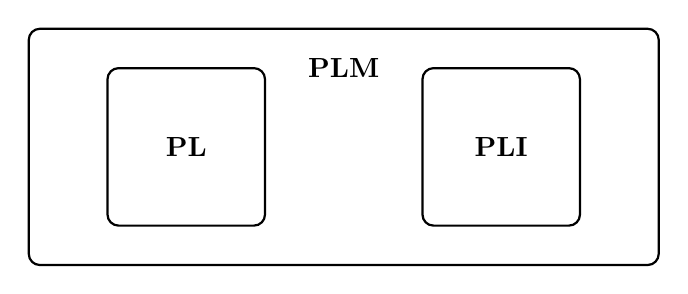
\begin{tikzpicture}
    
    \draw[thick, rounded corners] (-4, -1.5) rectangle (4, 1.5);
    
    \draw[thick, rounded corners] (-3, -1) rectangle (-1, 1);
    \node at (-2, 0) {\textbf{PL}};
    
    \draw[thick, rounded corners] (1, -1) rectangle (3, 1);
    \node at (2, 0) {\textbf{PLI}};
    
    \node at (0, 1) {\textbf{PLM}};
    
  \end{tikzpicture}
\end{center}
  
  


Un problema PL può sempre essere espresso nella seguente forma matriciale:
\[
  \max \{cx \mid Ax \leq b\}
\]
dove $ A \in \mathbb{R}^{m \times n} $ e $ b \in \mathbb{R}^m $. Grazie ad alcuni accorgimenti è possibile, inoltre, scrivere tutti i vincoli possibili di un problema di PL $\mathcal{P}$ in un'unico sistema di disequazioni lineari. Infatti:
\begin{itemize}
  \item Se \p è un problema di minimo, occorre considerare semplicemente la funzione $f (x) = (-c)x$
  \item Ogni vincolo $ax = b $diventa la coppia di vincoli $ax \leq b$ e $ax \geq b$
  \item Ogni vincolo $ax \geq b$ è equivalente a $(-a)x \leq (-b)$.
\end{itemize}

\subsection{Programmazione lineare intera}
Se nella $PL$ le variabili rappresentano quantità nella PLI le variabili possono essere
\begin{itemize}
  \item \textbf{Quantitative}: ovvero rappresentare quantità.
  \item \textbf{Logiche}: rappresentare valori booleani, ovvero scelte basate sulla possibilità di scegliere o meno una determinata opzione
\end{itemize}

Qui la definizione di variabile logica

\dfn{variabile logica}{
  Una \textbf{variabile} $x$ si definisce \textbf{logica} se:
  \[
    x \in \mathbb{N} (o \mathbb{Z}) \quad 0\leq x \quad x \leq 1
  \]
}

Un esempio tipico è rappresentato dalle variabili che associano una determinata risorsa a un compito specifico, oppure che determinano l'utilizzo di un particolare processo.

\begin{quote}
  Questo e' il bello dei problemi lineari

  \hfill -- Il Basta
\end{quote}

Un giga esempietto bellino è il problema dello zaino:
\ex{Problema dello zaino}{
  Il problema dello zaino è un esempio classico di problema di ottimizzazione combinatoria piuttosto complesso.

  % TODO: inserire il testo del problema
  TODO: inserire il testo del problema

  \vspace{1em}
  \textbf{Parametri:}
  \begin{align*}
    E &= \{1, \ldots, n\} \\
    a_i &= \text{peso dell'oggetto } i \\
    c_i &= \text{costo dell'oggetto } i \\
    b &= \text{peso massimo dello zaino}
  \end{align*}

  \vspace{1em}
  \textbf{Variabili:}
  \begin{align*}
  x_i &=
  \begin{cases}
  1 & \text{se l'oggetto } i \text{ è nello zaino} \\
  0 & \text{altrimenti}
  \end{cases} \\
  x_i &\in \{0, 1\} \quad \forall i \in \{1, \ldots, n\}
  \end{align*}

  \vspace{1em}
  \textbf{Vincoli:}
  \[
    \sum_{i=1}^{n} x_i a_i \leq b
  \]

  \vspace{1em}
  \textbf{Funzione obiettivo:}
  \[
    \max \sum_{i=1}^{n} x_i c_i
  \]

}

% Esempi di problemi di ottimizzazione lineari:
% \begin{itemize}
% \item Lo Zaino
% \item Albero di copertura minimo
% \item Commesso viaggiatore
% \end{itemize}

% \subsection{Problema dello Zaino}
% appunti scritti

\subsubsection{Relazioni logiche}

Avendo introdotto le variabili logiche, è opportuno chiedersi se sia possibile esprimere, mediante programmazione lineare (PL), le regole di inferenza logica per le relazioni che intercorrono tra di esse. Grazie all'uso di opportuni vincoli lineari, la risposta è affermativa:

\begin{itemize}
  \item \textbf{Negazione} \( (y = \neg x) \):
    \[
    x = 1 - y
    \]

  \item \textbf{Congiunzione} \( (z = x \land y) \):
    \[
    \begin{aligned}
      &z \leq x \\
      &z \leq y \\
      &z \geq x + y - 1
    \end{aligned}
    \]

  \item \textbf{Disgiunzione} \( (z = x \lor y) \):
    \[
    \begin{aligned}
      &z \geq x \\
      &z \geq y \\
      &z \leq x + y
    \end{aligned}
    \]

  \item \textbf{Implicazione} \( (z = x \implies y) \):
    \[
    \begin{aligned}
      &x + z \geq 1 \\
      &z \geq y \\
      &x + z \leq 1 + y
    \end{aligned}
    \]
\end{itemize}

È possibile, tuttavia, dimostrare che il problema di ottimizzazione lineare è, in generale, \textit{NP-hard}, dato che il problema di soddisfacibilità di una formula logica rientra nella classe NP-hard
\section{Template per risolvere problemi}

\subsection{Vincoli di assegnamento}
Un tipo di vincolo che la programmazione lineare intera (PLI) gestisce in modo molto efficace è rappresentato dai cosiddetti \textit{vincoli di assegnamento}. Questi vincoli sono utilizzati per modellare problemi che riguardano l'assegnazione di "oggetti a luoghi".

Si considerano:
\begin{itemize}
  \item Un insieme \( N = \{1, \ldots, n\} \) di \textbf{oggetti} (che possono rappresentare automezzi, persone, ecc.)
  \item Un insieme \( V = \{1, \ldots, m\} \) di \textbf{luoghi}
\end{itemize}

Per rappresentare le diverse condizioni di assegnazione degli oggetti ai luoghi, si introduce la variabile \( x_{ij} \in \{0, 1\} \) (dove \( 1 \leq i \leq n \) e \( 1 \leq j \leq m \)). Questa variabile indica se l'i-esimo oggetto è stato assegnato al j-esimo luogo (\( x_{ij} = 1 \)) o meno (\( x_{ij} = 0 \)), si può così procedere alla formale

\dfn{Vincoli di assegnamento}{
  Sia \( N = \{1, \ldots, n\} \) un insieme di oggetti e \( V = \{1, \ldots, m\} \) di luoghi, si definiscono \textbf{vincoli di assegnamento} quei vincoli che impongono che \textit{ogni oggetto sia assegnato a un solo luogo e ad ogni luogo è assegnato esattamente un oggetto}. Questi sono espressi mediante queste sommatorie:
  \[
    \sum_{j=1}^{m} x_{ij} = 1 \quad \forall i \in \{1, \ldots, n\} \quad \sum_{i=1}^{n} x_{ij} = 1 \quad \forall j \in \{1, \ldots, m\}
  \]

  Dove:
  \begin{itemize}
    \item \( x_{ij} \) è una variabile binaria che vale 1 se l'oggetto \( i \) è assegnato al luogo \( j \), e 0 altrimenti.
    \item La prima equazione assicura che ogni oggetto \( i \) sia assegnato esattamente a un luogo.
    \item La seconda equazione assicura che ogni luogo \( j \) riceva esattamente un oggetto.
  \end{itemize}
}

il luogo può anche essere visto come uno slot temporale, quindi imponiamo un certo pipeline


\subsubsection{Vincoli di semi-assegnamento}
I vincoli di semi-assegnamento sono una variante dei vincoli di assegnamento in cui non è necessario che ogni luogo riceva esattamente un oggetto, in particole si noti la seguente definizione

\dfn{Vincoli di semi-assegnamento}{
  Sia \( N = \{1, \ldots, n\} \) un insieme di oggetti e \( V = \{1, \ldots, m\} \) un insieme di luoghi. Si definiscono \textbf{vincoli di semi-assegnamento} quei vincoli che impongono che \textit{ogni oggetto sia assegnato ad al massimo un luogo}. Questi vincoli sono espressi mediante la seguente sommatoria:

  \[
  \sum_{j=1}^{m} x_{ij} \leq 1 \quad \forall i \in \{1, \ldots, n\}
  \]
  
  Dove \( x_{ij} \) è una variabile binaria che vale 1 se l'oggetto \( i \) è assegnato al luogo \( j \), e 0 altrimenti.
  

}


Insiemi ammissibili:

Vincoli di Assegnamento: ogni oggetto e' assegnato ad un luogo e ogni luogo ha un oggetto

\subsection{Selezione di Sottoinsiemi}

Sia $ N = \{1,...,n\} $ un insieme finito di elementi e sia $ F = \{F_1,...,F_n\} $ una famiglia di sottoinsiemi (non necessariamente disgiunti) dove $ F_i \subseteq N $. Vogliamo decidere qual'e' la scelta migliore di $ D\subseteq F $ di costo minimo. Per aiutare nella formulatzione del problema, possiamo rappresentare l'appartenenza degli ielementi di $ N $ in un sottoinsieme $ F_j $ come una grande matrice che ha come righe gli elementi e come colonne i sottoinsiemi. La scelta e' catturatanon piu' da $ x_{ij} $ ma solo da $ x_j $ dato che basta dire se il sottoinsieme $ j $ lo volgiamo o no. 
\[
x_j = \begin{cases}
1 & F_j \in D\\
0 & \text{altrimenti}
\end{cases}
\]

La funzione obbiettivo e' sempre:
\[
\sum_{j=1}^{n} x_j c_j
\]

I vincoli dipendono dal problema:
\begin{itemize}
\item Problema di copertura: ognuno degli eventi di $ N $ atanno in almeno uno degli elementi di $ D $:
  \[
  \sum_{j=1}^{m} a_{ij}x_j \geq 
  \]
    Numero di sottoinsiemi di $ D $ che appartengono a $ i $ (?). I sottoinsiemi $ F $ di $ N $ possono essere dei curriculum dove c'e' scritto quale dei linguaggi di programmazione $ n \in N $ conosce un candidato. Ogni candidato ha anche uno stipendio. Dobbiamo scegliere quali canditati assumere per coprire tutti i linguaggi in $ N $ minimizzando il costo.  
  \item Partizione: $ D $ deve essere una partizione di $ N $. $ N $ possono essere dei task da svolgere e gli iniemi di $ F $ sono offerte da fornitori rispetto alla risoluzione di alcuni dei task. Quindi gli inisiemi di $ D $ devono essere disgiunti perche' non vogliamo che due societa' risolvano lo stesso task. Tutto deve essere coperto una sola volta.
  \item Riempimento: si usa solo quando si vuole massimizzare. $ N $ non sono piu' incombenze o task, ma risorse da usare una volta per costruire un prodotto (elemento di $ F $). Al piu' perche' possiamo scartare qualche componente. Possiamo usare ogni elemento di $ N $ al massimo una volta. 
\end{itemize}

\ex{Problema delle Commesse}{
  Un'agenzia deve decidere come impiegare i soi $ n $ dipendenti.

  L'azienda, nell'intervallo di tempo considerato, deve evadere $ m $ commese.

  Ciascuna commessa $ j $ deve essere svolta dal sottoinsieme $ F_j \subseteq \{1,...,n\} $ dei dipendenti dell'azienda.

  Ogni commesssa, se evase, darebbe luogo ad un ricavo pari a $ r_j $.

  Ogni dipendente puo' lavorare ad una singola commessa nell'unita' di tempo.

  SVOLGIMENTO:

  e' un problema di selezione di sottoinsiemi:
  \[
  N - \{1,...,n\} \text{elementi/dipendenti}
  \]
  \[
  F = \{F_1,...,F_m\} commesse
  \]  

  VARIABILI:
  \[
  x_{j} = \begin{cases}
  1 & F_j \in D_j\\
  0 & \text{altrimenti}
  \end{cases}
  \]
  VINCOLI:
  $ 0\leq x_j \leq 1 \forall j $
  \[
  \sum_{j=1}^{m} x_j a_{ij} \leq 1 \forall i
  \]
  FO:
  \[
   \sum_{j=1}^{m} x_j r_j
 \]
 Ha fatto poi un esempio di quando c'e' una penalita' quando non fai una commessa (mi sa)
}

\subsection{Ricondurci a problemi linari}
Variabili a valori discreti possono prendere un insieme finito di valori diversi che non sono valori in un intervallo. Se questo insieme ha $ n $ valori ci servono $ n $ variabili diverse. 

\ex{Progetto di reti}{

}

alcune slide non le ho fatte

valore assoluto:
\[
  max \{f(x)| x \in X\} \quad max \{-f(x)|x \in X\}
\]
Abbiamo ridotto il problema che ha un valore assoluto a uno che non ce l'ha. Se ci fosse stata un operazione fra valori assoluti, la situa si complica

Funzioni lineari a tratti

in due dimensioni hanno la forma:
\[
  f(x) = \begin{cases}
    b_1 + c_1x & x \in [a_1, a_2]\\
    b_2+c_2x & x \in (a_2, a_3]
  \end{cases}
\]
nel punto $ a_2 $ ci puo' essere un punto di discontinuita'.

Come per il carico fisso vengono introdotte due variabili logiche asusiliarie $ y_1, y_2 $ co nil seguente significato:
\[
\]
Inoltre ci servono variabili ausiliarie che ci dicono lo spostamento rispetto a un estremo dell'intervallo a cui appartiene x:
\[
 
\]
Usiamo gli intervalli dinamici.
\[
 
\]
Non c'e' niente che ci da la funzione da ottimizzare, abbiamo solo delle definizioni che sono dei semplici commenti, i vincoli lineari sono solo gli ultimi, ma non bastano. 

Rappresentiamo la funzione $ f $ con una funzione $ g $ che prende le variabili logiche e quantitative. 
\[

\]
Il valore di $ f $ e' rappresentato univocamente dalla quadrupla, eccetto nel punto di non continuita'. Solo il primo valore e' accettabile perche' l'intervallo li e' chiuso. 

GNU MathProf




% \begin{document}
\chapter{Reti di Flusso}

Innanzi tutto inziamo con alcune definzioni:
\dfn{Rete}{
  definiamo \textbf{rete} un grafo \textit{pesato} $ G = (N,A) $ dove
  \begin{itemize}
    \item $ N $ e' l'insieme dei nodi
    \item $ A $ e' l'insieme degli archi
  \end{itemize}
}

Più precisamente:
\begin{itemize}
  \item $\forall i \in N$ è associato un valore reale $b_i$, detto \textit{sbilanciamento} che può essere:
  \begin{itemize}
    \item \textbf{Positivo}: il nodo $i$ è detto \textit{pozzo} e rappresenta la qunatità del bene che esce della rete al nodo $i$, mentre $b_i$ è ldetto \textit{domanda del bene}
    \item \textbf{Negativo}: il nodo $i$ è detto \textit{sorgente} e rappresenta la quantità del bene che entra nella rete al nodo $i$, mentre $-b_i$ è detto \textit{offerta del bene}
    \item \textbf{Nullo}: il nodo $i$ è detto \textit{transito} e rappresenta un nodo di passaggio
  \end{itemize}
  \item $\forall (i,j) \in A$ è associato un valore reale $c_{ij}$ detto \textit{costo} che rappresenta il costo di trasportare una unità di bene lungo l'arco $(i,j)$ ed una coppia di valori $l_{ij}$ e $u_{ij}$ detti \textit{capacità inferiore} e \textit{capacità superiore} rispettivamente, che rappresentano il minimo e il massimo numero di unità di bene che possono essere trasportate lungo l'arco $(i,j)$
  \begin{center}
    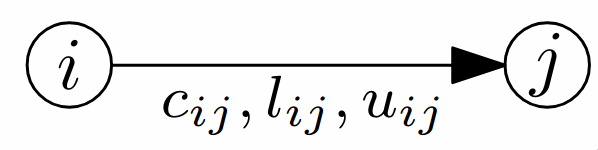
\includegraphics[width=0.5\textwidth]{img/2025-03-05-09-34-49.png}
  \end{center}
\end{itemize}

\section{Problemi di Flusso}
\dfn{Problemi di flusso}{
  > Si definiscono \textit{problemi di flusso} quei problemi che consistono nel determinare, lungo una rete, il flusso di un bene, ossia un assegnamento a ciascun arco \( (i,j) \in A \) un valore reale \( x_{ij} \in [l_{ij}, u_{ij}] \), rispettando i vincoli di capacità e conservazione del flusso
}

\textbf{flusso}, quindi, e' proprio la soluzione che vogliamo trovare. Tuttavia ad ogni unità di flusso assegnata ad un arco corrisponde un costo $c_{ij}$, si ha quindi che il costo complessivo del flusso e' dato da:
\begin{equation}  
  \sum_{(i,j) \in A} c_{ij}x_{ij}
\end{equation}


\subsection{Vincoli}
I vincoli che nei problemi di flusso si deve rispettare sono:
\begin{itemize}
\item \textit{Uguaglianza di domanda e offerta globale}:
  \begin{equation}
    \sum_{i \in D}b_i = - \sum_{i \in O} b_i \iff \sum_{i \in N} b_i = 0
  \end{equation}
  Dove $ D = \{b_i \in N \mid b_i > 0\} $ e $ O = \{b_i \in N \mid b_i < 0\} $. Per quelli nulli, tanto vale non metterli da nessuna parte per non creare asimmetria inutile.
\item \textit{Conservazione di flusso}:
  \begin{quote}
    lol 
    \hfill \textit{Il Basta}
  \end{quote}

  \begin{equation}
    \sum_{(i,j) \in BS(i)} x_{ij} - \sum_{(i,j) \in FS(i)} x_{ij} = b_i \quad \forall i \in N
  \end{equation}
  
dove
\begin{align*}
  BS(i) = \{(k,i) | (k,i) \in A\} \text{ detto stella entrante}\\
  FS(i) = \{(i,k) | (i,k) \in A\} \text{ detto stella uscente}
\end{align*}
Ovvero ciò che entra nel nodo e' uguale a cio' che esce piu' lo sbilanciamento.
\item \textit{Ammissibilità del flusso}:
  \[
    l_{ij} \leq x_{ij} \leq u_{ij} \quad \forall (i,j) \in A
  \]
\end{itemize}



\ex{Esempio di rete}{
  \begin{center}
    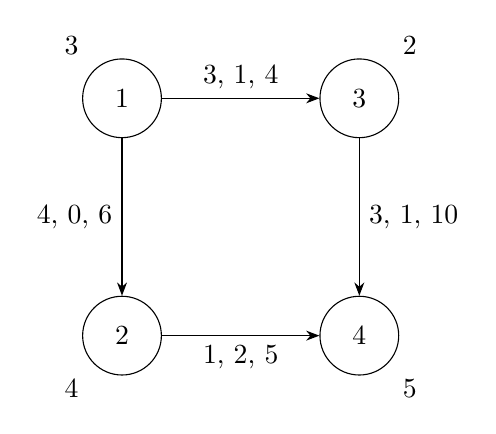
\begin{tikzpicture}[
        node distance=2cm,
        vertex/.style={circle, draw, minimum size=1cm},
        edge/.style={->, >=Stealth, auto},
    ]

    % Nodes
    \node[vertex] (1) {1};
    \node[vertex, below=of 1] (2) {2};
    \node[vertex, right=of 1] (3) {3};
    \node[vertex, below=of 3] (4) {4};

    % Edges
    \draw[edge] (1) -- node[above] {3, 1, 4} (3);
    \draw[edge] (1) -- node[left] {4, 0, 6} (2);
    \draw[edge] (2) -- node[below] {1, 2, 5} (4);
    \draw[edge] (3) -- node[right] {3, 1, 10} (4);

    % Labels
    \node[above left=0.1cm of 1] {3};
    \node[below left=0.1cm of 2] {4};
    \node[above right=0.1cm of 3] {2};
    \node[below right=0.1cm of 4] {5};

    \end{tikzpicture}
  \end{center}  
}

Perche' mai dovremmo studiare sta roba? 
\begin{itemize}
\item \textbf{Espressivita'}: permette di catturare un range di problemi concreti abbastanza grande
\item \textbf{Complessita'}: esistono algoritmi che risolvono questo tipo di problemi con complessita' polinomiale abbastanza basso. A Ugo questo fa molto piacere :), perché ricordiamolo NON SIAMO INGENERI GESTIONALI, SIAMO INFORMATICI
\end{itemize}

\subsection{Ipotesi semplificative}

Le ipotesi semplificative sono supposizioni che non consentono di usare il caso generale, ma che semplificano il problema \textbf{senza} perdere espressivita', come ad esempio nel caso in cui le capacita' inferiori sono nulle ovvero $l_{ij}=0$, che e' una situazione a cui possiamo arrivare \textbf{anche da grafi che non hanno questa caratteristica}. 

Infatti data una rete $G$, si può costruire una rete $G'$ tale che $G$ e $G'$ hanno lo stesso flusso ottimo, ma $G'$ ha capacita' inferiori nulle. $\forall (i,j)\in A$:
\begin{itemize}
\item Si sottrae $ l_{ij} $ a $ b_j $ e a $ u_{ij} $
\item Si aggiunge $ l_{ij} $ a $ b_i $
\item Occorre aggiungere la quantita'
  \[
    \sum_{(i,j) \in A} c_{ij}l_{ij}
  \]
  Alla funzione abbiettivo 
\end{itemize}
\nt{
  Si noti che non cambia la soluzione ottima, ma solo il valore ottimo della funzione obbiettivo
}

È pertanto vero, quindi, che ad un flusso $x_{ij} \in G $ corrisponde un flusso $(x_{ij}+l_{ij}) \in G'$
\subsection{Problema del Flusso di Costo Minimo}

\dfn{Problema del Flusso di Costo Minimo}{
  Si definisce \textit{problema del flusso di costo minimo} il problema di flusso in cui la funzione obbiettivo è il costo di flusso da minimizzare e le cui capacità inferiori sono nulle
}

Questo problema è formalizzabile in programmazione lineare come segue:
\begin{equation}
  \begin{aligned}
    \min &cx\\ 
    Ex &= b \quad \leq x \leq u  
  \end{aligned}
\end{equation}
dove

\begin{itemize}
  \item $x \in \mathbb{R}^{|A|} $ è il vettore delle variabili di flusso
  \item $c \in \mathbb{R}^{|A|} $ è il vettore dei costi
  \item $E \in \mathbb{R} ^{|N| \times |A|} $ e' una matrice di incidenza fra nodi e archi i cui elementi possono solo assumere valori 0, -1 e 1
  \item $b \in \mathbb{R}^{|N|} $ e' il vettore degli sbilanciamenti
  \item $u \in \mathbb{R}^{|A|}$ e' il vettore delle capacita' superiori
\end{itemize}

In questo modo abbiamo scritto funzione obbiettivo e vincola in forme matriciali molto semplici, adesso, senza terrorizzare nessuno, fornirò la formalizzazione in forma estesa:
\begin{equation}
  \begin{aligned}
    \min &\sum_{(i,j) \in A} c_{ij}x_{ij}\\
    &\sum_{(j,i)\in BS(i)}x_{ji} -\sum_{(i,j) \in A} x_{ij} = b_i \quad \forall i \in N\\
    &l_{ij} \leq x_{ij} \leq u_{ij} \quad \forall (i,j) \in A
  \end{aligned}
\end{equation}

\subsubsection{Rilassamento di assunzioni}
Puo' essere utile assumere che esiste un solo pozzo e una sola sorgente, che vengono poi collegati con archi fittizi (a costo nullo e capacita' pari allo sbilanciamento dei pozzi/sorgenti effettivi!) a quelli effettivi. 

Per trasformare un generico problema MCF in un problema con una sola sorgente ed un solo pozzo$ \dots $
\begin{itemize}
  \item Si aggiungono due nodi fittizi $s$ e $t$, uno sorgente e uno pozzo
  \item Si aggiungono archi fittizi  da $s$ ai nodi sorgenti di partenza, con un costo nullo e capacita' pari all'inverso dello sbilanciamento del nodo sorgente, ovvero $-b_s$
  \item Si aggiungono archi fittizi dai nodi pozzo ai nodi pozzo di arrivo, con un costo nullo e capacita' pari allo sbilanciamento del nodo pozzo
  \item Lo sbilanciamento di $s$ e' pari alla somma degli sbilanciamenti dei nodi sorgenti, mentre lo sbilanciamento di $t$ e' pari alla somma degli sbilanciamenti dei nodi pozzo
\end{itemize}

\ex{Esempio di Rilassamento}{
  Si parte da questa rete:
  \begin{center}
    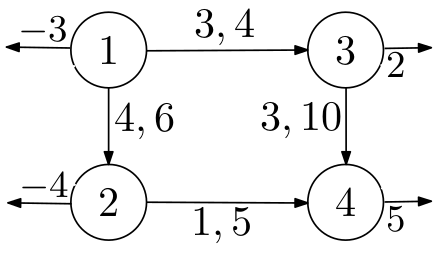
\includegraphics[width=0.5\textwidth]{img/rete_non_rilassata.png}
  \end{center}
  Si aggiungono i nodi fittizi $s$ e $t$ con sbilanciamento rispettivamente $b_s =b_1+b_2=-3-4 =-7$ e $b_t = b_3+b_4 = 2+5 =7$

  Si aggiungono gli archi fittizi con costo nullo e con capacità:
  \begin{itemize}
    \item $a_{s1} = -b_1 = 3$
    \item $a_{s2} = -b_2 = 4$
    \item $a_{3t} = b_3 = 2$
    \item $a_{4t} = b_4 = 5$
  \end{itemize}

  Si ottiene quindi la seguente rete rilassata:
  \begin{center}
    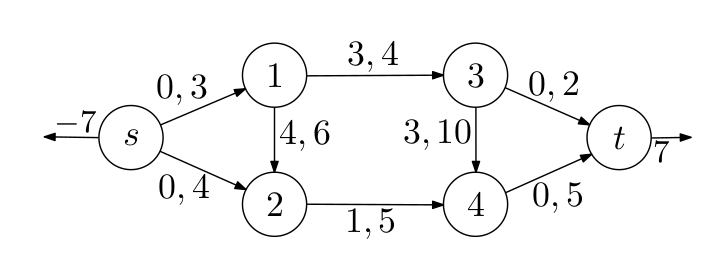
\includegraphics[width=0.5\textwidth]{img/rete_rilassata.png}
  \end{center}
}
\begin{quote}
  Non si può, però, enunciare che i nodi non hanno una capacita', perche' di fatto non succede nulla, perche' puo' essere trasformata in una rete equivalente dove i nodi non ce l'hanno:

  \hfill \textit{TODO: spiegare meglio, che cazzo vuoi dire ibbastianini?}

  Mi spiego in modo piu' eloquente: Per poter utilizzare nodi che hanno una propria capacita', non e' necessario perdere generalita' cambiando la definizione del problema esaminato. Questo e' vero, in quanto una tale rete puo' essere banalmente trasformata in una rete equivalente la quale presenta solo nodi con capacita' nulla. Come accade tale trasformazione? Facciamocelo spiegare da GioPalmi:
\end{quote}

Alle volte, inoltre, è utile che anche i nodi abbiano delle \textbf{capacità}, ossia che solo che solo una quantità di flusso compresa nell’intervallo chiuso $[l_i , u_i]$ possa passare per il nodo $i \in N$. Per fare ciò occorre \textit{sdoppiare} ciascun nodo $i$ in due nodi $i',i''$, in modo che:
\begin{itemize}
  \item Tutti gli archi entranti in $i$ entrino in $i'$ 
  \item tutti gli archi uscenti da $i$ escano da $i''$
  \item Si aggiunge un arco da $i'$ a $i''$ con capacità $[l_i,u_i]$
\end{itemize}
\begin{center}
  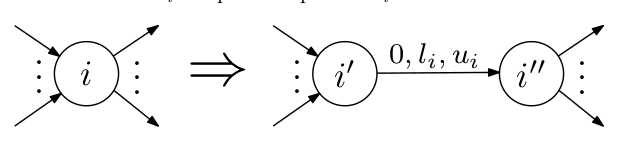
\includegraphics[width=0.5\textwidth]{img/giga_archetto_con_capacity.png}
\end{center}

\subsection{Problema di Flusso Massimo}

\dfn{Problema di Flusso Massimo}{
  Dato un grafo $ G = (N,A) $ orentato su cui definiamo:
  \begin{itemize}
  \item il vettore di capacita' superiori $ u = [u_{ij}] $ associate agli archi
  \item $ s $ (\textit{origine} o \textit{sorgente}) e $ t $ (\textit{destinazione} o \textit{pozzo}) due nodi distinti
  \end{itemize} 
  si definisce \textit{problema di flusso massimo} il problema di massimizzazione del flusso da $ s  $ a $ t $.

  Ovvero, il problema consiste nel trovare il \textbf{massimo} valore $ v $ tale che se $ b_s = -v $, $ b_t = v $ e per tutti gli altri casi $ b_i = 0 $, allora esiste un flusso $ x = [x_{ij}] $ ammissibile. Tale $ v $ si dice \textbf{valore} del flusso $ x $.
}
Ciò che cambia, quindi, dal problema di flusso di costo minimo è la funzione obbiettivo, che diventa, si vuole infatti \textit{massimizzare} il flusso, e non minimizzare il costo (che non ci interessa). 

Formalizzato in programmazione lineare, il problema di flusso massimo diventa:
\begin{equation} \label{PL_FM}
  \begin{aligned}
  \max \quad & v \\
  \sum_{(j,s) \in BS(s)} x_{js} + v &= \sum_{(s,j) \in FS(s)} x_{sj}; \\
  \sum_{(j,i) \in BS(i)} x_{ji} - \sum_{(i,j) \in FS(i)} x_{ij} &= 0, \quad i \in N - \{s, t\}; \\
  \sum_{(j,t) \in BS(t)} x_{jt} &= \sum_{(t,j) \in FS(t)} x_{tj} + v; \\
  0 \leq x_{ij} &\leq u_{ij}, \quad (i,j) \in A.
  \end{aligned}
\end{equation}

\nt{
  Si noti che il problema di flusso massimo e' un caso particolare di problema di flusso di costo minimo. Difatti la formulazione \ref{PL_FM} puo' essere vista come la descrizione di un problema di MCF su un grafo $ G' $ ottenuto da $ G $ con delle modifiche: 
  \begin{itemize}
    \item Si aggiunge un arco fittizio $ (t,s) $, detto \textit{arco di ritorno}, con capacita' infinita.
    \item Tutti i nodi sono di trasferimento ($ \forall i \in N.\ b_i = 0 $), si tratta quindi di un problema di \textit{circolazione}.
    \item Tutti i costi degli archi sono nulli tranne $ (t,s) $ che ha costo $ -1 $.
  \end{itemize}

  Di conseguenza, risolvendo il problema di MCF su $ G' $, stiamo minimizzando il valore $ -1 \cdot x_{ts} $ rispettando i vincoli imposti, che per definizione corrisponde a $ -v $. Ma minimizzare $ -v $ significa massimizzare il valore $ v $ del flusso fra $ t $ ed $ s $, che  e' proprio l'obbiettivo del problema di MF.
}

\ex{Risolvere un problema MF come MCF}{ \label{ex:FM}
  Dato il seguente problema di MF, con capacita' superiori indicate in figura e dove i nodi diversi da $ s $ e $ t $ hanno sbilanciamento nullo (come per definizione del problema), trasformarlo in un problema MCF:
  \begin{center}
    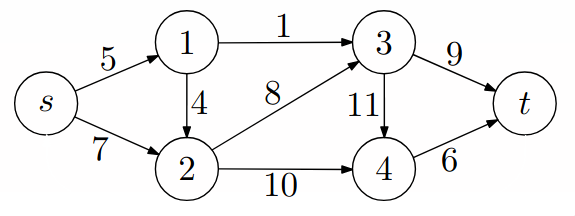
\includegraphics[width=0.5\textwidth]{img/2025-03-13-11-01-34.png}
  \end{center}

  Il problema di MF consiste nel determinare il massimo valore di flusso $ v $, ovvero il massimo valore di sbilanciamento uguale per $ s  $ (ma con segno meno) e $ t $ (devono essere per forza uguali per il vincolo di \textit{uguaglianza di domanda e offerta globale}) per cui esiste un flusso ammissibile $ x = [x_{ij}] $ (che quindi rispetta i vincoli di \textit{ammissibilita'} e di \textit{conservazione}). 

  A prima occhiata, possiamo subito dire che il valore limite per $ v $ e' sicuramente $ 5 + 7 = 12 $, dato che per il vincolo di conservazione $ b_s = x_{s1} + x_{s2} \leq u_{s1} + u_{s2} $ (facendo lo stesso ragionamento con $ t $, otteniamo un limite meno stringente, quindi prevale questo). Siamo sicuri che $ v = 0 $ sara' sempre una soluzione ammissibile, dato che $ x = \underline{0} $ e' sempre un flusso ammissibile, ma non e' quasi mai il valore massimo. Facciamo i passi con $ v = 12 $:
  \begin{itemize}
  \item Dobbiamo mettere $ x_{s1} = 5 $ e $ x_s2 = 7 $
  \item Dobbiamo mettere $ x_{13} = 1 $ e $ x_{12} = 4 $
  \item Ora abbiamo che $ \sum_{(j,i) \in BS(2)} x_{ji} = 7 + 4 = 11 $ e dobbiamo decidere come dividere il flusso entrante fra quelli uscenti, dato che questa volta non vengono saturati. Possiamo usare l'euristica e guardare i nodi di destinazione: il 3 ha capacita' superiori per i flussi uscenti rispetto al nodo 4, quindi gli mandiamo piu' flusso possibile (questa e' solo un'intuizione e non e' affatto una regola generale). Quindi $ x_{23} = 8 $ e $ x_{24} = 3 $.
    \item Poniamo $ x_{3t} = 9 $ e $ x_{4t} = 3 $: esiste un flusso $ x $ ammissibile per $ v = 12 $! E dato che 12 e' il limite massimo, siamo sicuri che e' la soluzione al problema.
  \end{itemize}

  Non sempre sara' cosi' facile trovare la soluzione corretta. Vediamo il problema MCF corrispondente e convinciamoci che e' equivalente:
  \begin{center}
    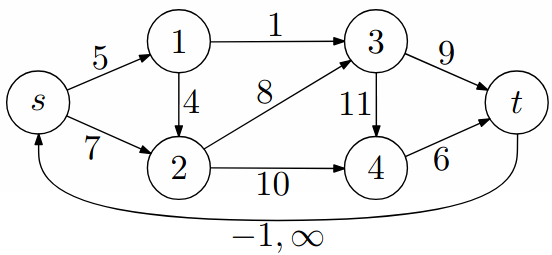
\includegraphics[width=0.5\textwidth]{img/2025-03-13-11-38-15.png}
  \end{center}

Le capacita' massime sono uguali, tutti i nodi hanno sbilanciamento nullo e abbiamo aggiunto l'arco di ritorno. La funzione obbiettivo e:
\[
min -x_{ts} \equiv max x_{ts}
\]
dato che tutti gli altri costi sono nulli. Dato che $ s  $ e $ t $ hanno sbilanciamento nullo, per i vincoli di conservazione e di ammissibilita':
\[
x_{ts} = x_{3t} + x_{4t} \leq u_{3t} + u_{4t} = 15 \quad \land \quad u_{s1} + u_{s2} = 12 \geq x_{s1} + x_{s2} = x_{ts}
\]
da qui otteniamo che $ x_{ts} \leq 12 $ e' il limite superiore. Da questo punto, controllare se con $ x_{ts} = 12 $ possiamo costruire un flusso ammissibile segue lo stesso identico procedimento di prima. Quindi il flusso che minimizza il costo e' proprio $ x $ il cui valore di flusso associato $ v = x_{ts} $ e' il valore della soluzione MF.
}
  
\section{Problema del flusso massimo: algoritmi}
Abbiamo capito quindi che il problema di Flusso Massimo e' un problema di MCF con due caratteristiche specifiche:
\begin{itemize}
\item Il vettore dei bilanci $ b $ e' nullo
\item Il vettore dei costi $ c $ e' nullo tranne per $ c_{ts} $ che vale $ -1 $
\end{itemize}
Vediamo come queste caratteristiche permettono di utilizzare algoritmi specifici al problema, che sono molto piu' veloci di quelli generali.

\subsection{Tagli}

\dfn{Taglio}{
  Si definisce \textbf{taglio} in una rete $G=(N,A)$ una coppia $(N',N'')$ di sottoinsiemi di $N$ tali che $N' \cup N'' = N$ e $N' \cap N'' = \emptyset$
}

Si noti, inoltre anche questa defnizione
\dfn{$(s,t)$-taglio}{
  Si definisce \textbf{$(s,t)$-taglio} in una rete $G=(N,A)$ un taglio ($N_s, N_t$) dove $s \in N_s$ e $t \in N_t$
}

Si prendi in considerazione inoltre i confini il confine fra gli $(s,t)-\text{tagli}$, dove:
\begin{itemize}
  \item $A^+(N_s, N_t) = \{(i,j) \in A \mid i \in N_s \land j \in N_t\}$ sono gli archi che vanno dalla partizione $s$ a $t$
  \item $ A^-(N_s,N_t)=\{(i,j)\in A\mid i\in N_t\land j\in N_s\} $ sono gli archi che vanno da $t$ a $s$
\end{itemize}

\ex{Taglio (s,t) di un problema di flusso massimo}{
  Ecco un esempio di taglio (rappresentato dalla riga blu) che partiziona in due sottoinsiemi i nodi di un problema di flusso massimo:
  \begin{center}
    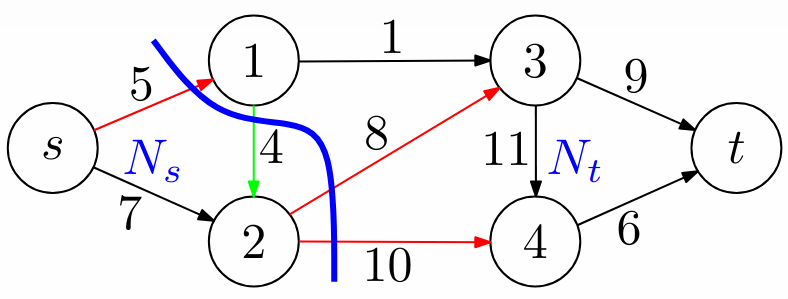
\includegraphics[width=0.5\textwidth]{img/2025-03-13-18-25-02.png}
  \end{center}
  Dal grafo si deduce che:
  \begin{itemize}
  \item $ N_s = \{s,2\} $
  \item $ N_t = \{1,3,4,t\} $
  \item $ A^{+} = \{(s,1), (2,3), (2,4)\} $
  \item $ A^{-} = \{(1,2)\} $
  \end{itemize}
}

Adesso introduciamo un importante lemma sui tagli:
\mlenma{}{
  $\forall (s,t)-\text{taglio }(N_s,N_t)$ e $\forall$ flusso ammissibile $x$ con valore $v$, si ha che:
  \begin{itemize}
    \item $v = \sum_{(i,j)\in A^+(N_s,N_t)}x_{ij}- \sum_{(i,j)\in A^-(N_s,N_t)}x_{ij}$
    
    Si ha, quindi, che $v$ la somma del flusso uscente da $s$ meno il flusso entrante in $s$.     Questa quantità è detta \textbf{flusso del taglio} $(N_s, N_t)$ e la si denota $x(N_s, N_t)$

    \item $v\leq \sum_{(i,j)\in A^+(N_s, N_t)} u_{ij}$
    
    Ovvero Il flusso massimo è sempre minore o uguale alla capacità totale del taglio. Questa quantità è detta \textbf{capacità del taglio} ed è indicata con $u(N_s, N_t)$
  \end{itemize}
}
\pf{Dimostrazione}{
  \begin{itemize}
    \item Dimostro la prima parte:
    Per definizione di $v$, si ha che:
    \[
      v = \sum_{(s,j)\in A}x_{sj} - \sum_{(i,s)\in A}x_{is}
    \]
    
      
    Questo valore è uguale alla somma netta in uscita $\forall i\in N_s$ verso la partizione $N_t$, quindi:
      \footnote{
        Possiamo dimostrare questa cosa dato che, per il vincolo di conservazione e per definizione del problema:
      \[
        \forall k \in N_s.\ \sum_{(k,j) \in A} x_{kj} - \sum_{(i,k)} x_{ik} = \begin{cases}
        v & k = s \\
        0 & k \neq s 
        \end{cases}
      \]
      }
    \[
      \sum_{(i,j)\in A}x_{ij} - \sum_{(i,j)\in A}x_{ji} = \sum_{k\in N_s}\left( \sum_{(k,j)\in A}x_kj-\sum_{(i,k)\in A}x_{ik} \right)
    \]
    Riscrivendo usando la proprieta' distributiva, posso dividere l'esspressione in due parti:
      \[
        \underbrace{\sum_{k \in N_s} \sum_{(k,j) \in A} x_{kj}}_\text{somma archi uscenti $ S^{+} $} - 
        \underbrace{\sum_{k \in N_s} \sum_{(i,k)} x_{ik}}_\text{somma archi entranti $ S^{-} $}
      \]
      Dato che $ k \in N_s $, consideriamo tutti gli archi $ (p,q) $ che hanno \textit{almeno} un nodo dentro a $ N_s $, ci sono quindi tre casi:
      \[
      \begin{cases}
        p \in N_s \land q \in N_t & \to S^{+} \mathrel{+}= x_{pq} \\
        p \in N_t \land q \in N_s &  \to S^{-} \mathrel{+}= x_{pq} \\
        p,q \in N_s & \to S^{+} \mathrel{+}= x_{pq} \land S^{-} \mathrel{+}= x_{pq}
      \end{cases}
      \]
      Ma aggiungere lo stesso valore in $ S^{+} $ e in $ S^{-} $ non ha effetto sul valore finale dato che si annullano, quindi possiamo anche non considerare gli archi fra nodi che appartengono a $ N_s $. 

      Consideriamo quindi solo gli archi che attraversano il taglio: $ S^{+} $ e' la somma dei flussi da $ N_s $ a $ N_t $ e $ S^{-} $ i flussi da $ N_t $ a $ N_s $. Quindi la loro somma e' uguale al flusso uscente dal confine $A^+(N_s, N_t)$ meno il flusso entrante dal confine $A^-(N_s, N_t)$, allora:
    \[
      \sum_{k\in N_s}\left( \sum_{(k,j)\in A}x_kj-\sum_{(i,k)\in A}x_{ik} \right) = \sum_{(i,j)\in A^+(N_s,N_t)}x_{ij}- \sum_{(i,j)\in A^-(N_s,N_t)}x_{ij}
    \]
  
    Per riassumere quindi:
    \begin{equation}
      v = \sum_{(i,j)\in A^+(N_s,N_t)}x_{ij}- \sum_{(i,j)\in A^-(N_s,N_t)}x_{ij}
    \end{equation}
    \item Dimostro la seconda parte:
    
    Ovvio perché è una semplice derivazione del punto 1
  \end{itemize}
}

\nt{
  si noti che la conclusione di questo Lemma è
  \[
    v = x(N_s, N_t)\leq u (N_s, N_t)
  \]

  Ovvero \textit{il valore di un flusso ammissibile è sempre minore o uguale della capacità di qualunque taglio}. 
}
\nt{
  Abbiamo utilizzato il secondo punto del lemma all'esempio \ref{ex:FM}, quando abbiamo imposto un limite superiore al valore di $ v $ sommando le capacita' massime degli archi uscenti da $ s  $ e poi con gli archi entranti a $ t $. Quindi e' come se avessimo costruito un taglio con $ N_s = \{s \} $ e uno con $ N_t = \{t\} $, per poi imporre il secondo punto del lemma, scegliendo quello minore come limite. 

  Pero' abbiamo controllato solo due tagli specifici, quello che aggiunge il lemma e' che tale proprieta' vale per tutti i tagli, quindi per trovare un limite migliore tocca calcolare la capacita' di tutti i tagli possibili.
}

Adesso tratteremo il caso un cui si voglia determinare se esiste un taglio con capacità \textbf{identica} al valore di un flusso ammissibile (ovvero massimo)

\subsection{Cammini aumentanti e Grafo residuo}
Innanzi tutto dobbiamo presentare alcuni concetti


\subsubsection{Cammino aumentante}
Dato una rete di un problema di MF e un suo flusso ammissibile, noi vogliamo sapere se questo flusso e' ottimo. Se non fosse ottimo, cio' significa che sarebbe possibile inviare altro flusso da $ s $ a $ t $, che quindi dovra' seguire un certo cammino $ P $. Tale cammino non segue per forza l'orientamento del grafo, quindi e' possibile che un arco $ (i,j) $ venga attraversato al contrario. Provo a dare l'intuizione del perche' con un esempio:
\ex{}{
  Consideriamo il seguente grafo (ignorare il taglio):
  \begin{center}
    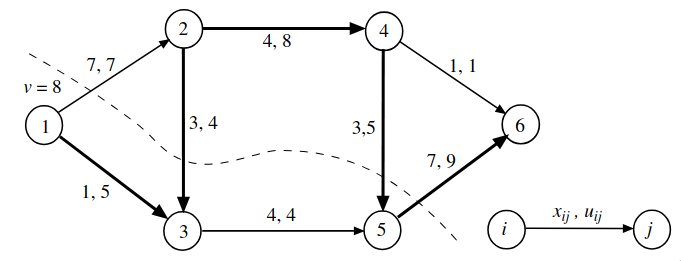
\includegraphics[width=0.5\textwidth]{img/2025-03-13-21-24-42.png}
  \end{center}
  Attualmente, il valore del flusso vale 8. Vogliamo vedere se e' possibile aumentare il flusso. Proviamo ad aumentare il flusso di 2 ($ v = 10 $):
  \begin{itemize}
    \item Dato che l'arco $ (1,2) $ e' saturo, devo aumentare $ x_{13} $ di 2
    \item L'unico arco uscente da 3 e' saturo, quindi non possiamo far proseguire il flusso. Puo' sembrare di essere in un vicolo cieco, perche' dove lo mettiamo questo flusso in piu'? Ma, come abbiamo detto prima, il cammino che stiamo cercando \textit{non e' per forza orientato}, quindi sarebbe possibile "proseguire" lungo l'arco $ (2,3) $ al contrario. Questo e' perche' in questa situazione possiamo fare una giocata: il nodo 3 e' sovraccaricato, dato che il flusso non puo' uscire da nessuna parte, quindi dobbiamo diminuire quello in entrata. Il flusso $ x_{13} $ appena aumentato lo vogliamo tenere, dato che fa parte del percorso, quindi \textit{diminuiamo} il flusso $ x_{12} $ della stessa quantita' di quanto abbiamo aumentato il flusso dell'arco entrante. In questo modo il totale di flussi entranti al nodo 3 rimane uguale, ma il nodo 2 ha ora ben 2 di flusso in piu' che puo' utilizzare! Quindi, il flusso in piu' che vogliamo far arrivare a 6 si e' spostato da 3 a 2, ed e' proprio per questo che possiamo attraversare gli archi al contrario. Ma attenzione, al posto di aumentare il valore del flusso $ x_{23} $, l'abbiamo diminuito, cosa che definiremo meglio dopo.
    \item Ora che il nodo 2 ha del flusso extra, lo inviamo al nodo 4 ($ x_{24} += 2 $)
    \item Il nodo 4 lo manda al nodo 5 che infine lo manda al nodo 6.
  \end{itemize}
  Notare che se avessimo scelto di aumentare $ v $ di 3, dal nodo 4 non sarebbe stato possibile rispettare i vincoli di ammissibilita', quindi il valore 2 non era scelto a caso.
}

Ora che e' chiaro cosa stiamo cercando e perche', iniziamo a formalizzare le intuizioni. Per prima cosa, distinguiamo gli archi attraversati col verso "giusto" da quelli attraversati con verso "opposto":
\dfn{Archi concordi e discordi}{
  Dato un cammino $ P $ su una rete $ G $, chiamiamo:
  \begin{itemize}
  \item L'insieme degli archi \textit{conocrdi} $ P^{+} $ l'insieme degli archi del percorso $ P $ che hanno lo stesso orientamento degli archi corrispondenti in $ G $
  \item L'insieme degli archi \textit{discordi} $ P^{-} $ l'insieme degli archi del percorso $ P $ che hanno verso opposto rispetto agli archi corrispondenti in $ G $
  \end{itemize}
}

\ex{}{
  Quindi, nell'esempio di prima:
  \begin{itemize}
    \item $ P^{+} = \{(1,3), (2,4), (4,5), (5,6)\} $
    \item $ P^{-} = \{(3,2)\} $
  \end{itemize}
}

Definiamo ora la capacita' di un percorso, che dimostreremo essere la quantita' in piu' di flusso che tale percorso puo' portare da $ s  $ a $ t $:
\dfn{Capacità di un cammino}{
  Dato un cammino $P$ in una rete $G$ rispetto a un flusso $x$, la \textbf{capacità} di $P$ rispetto a $x$ è definita come:
  \begin{equation}
    \theta (P,x) = \min{\{\min{\{u_{ij}-x_{ij}\mid (i,j)\in P^+\}},\min{\{x_{ij}\mid (j,i)\in P^-\}}\}}
  \end{equation} 
}

\nt{
  Quindi abbiamo definito $ \theta(P,x) $ in questo modo per fare in modo che corrisponda alla quantita' massima di flusso che possiamo mandare in piu' rispetto al flusso OG $ x $ in modo che rimanga sempre ammissibile. Notare che e' possibile che tale valore sia nullo, nel caso in cui uno degli archi concordi e' saturo o uno di quelli discordi e' nullo, in questo caso $ P $ non e' aumentante.
}

Dalla definizione di capacita' discende la definizione di flusso $x(P,\theta)$:
\dfn{Flusso $x(P,\theta)$}{
  Dato un cammino aumentante $P$ in una rete $G$ rispetto a un flusso $x$ e una capacità $\theta$, il flusso $x(P,\theta)$ è definito come:
  \begin{equation}
    (x(P,\theta))_{ij} = 
    \begin{cases}
      x_{ij}+\theta & (i,j)\in P^+\\
      x_{ij} - \theta & (i,j)\in P^-\\
      x_{ij} & \text{altrimenti}
    \end{cases}
  \end{equation}
}

\mlenma{}{
  Se $ x $ e' ammissibile, allora anche $ x(P, \theta(P, x)) $ e' ammissibile
}
\pf{}{
  TODO: dimostra (facile)
}

Possiamo ora definire un cammino aumentante come:
\dfn{Cammino aumentante}{
  Data una rete $ G $ di un problema MF, un cammino da $ s  $ a $ t $ \textit{non necessariamente orientato} si dice \textbf{aumentante} se $ \theta(P,x) > 0 $.
}

\subsubsection{Grafi residui}

Per definire un algoritmo che riesca a determinare se esisti o meno un cammino aumentante dato un grafo $ G $ e un flusso ammissibile $ x $, ci e' piu' comodo lavorare su sul cosidetto \textit{grafo residuo} $ G_x $ associato: 
\dfn{
  grafi residui
}{
  Dati una rete $G =(N_G, A_G)$ ed un flusso ammissibile $x$ si definisce il \textbf{grafo residuo} $G_x$ il multigrafo $(N_{G_x}, A_{G_x})$ tale che:
  \begin{itemize}
    \item $N_{G_x} = N_G$
    \item Gli archi in $A_{G_x}$ sono di due tipi:
    \begin{itemize}
      \item $\forall (i,j)\in A_G$ tale che $x_{ij}<u_{ij}$ esiste un arco da $i$ a $j$ in $G_x$ detto \textbf{arco concorde}
      
      Signifca che il flusso non ha saturato la capicità dell'arco e si può ancora inviare flusso in quella direzione
      \item $\forall (i,j)\in A_G$ tale che $x_{ij}> 0$ esiste un arco da $j$ a $i$ in $G_x$ detto \textbf{arco discorde}
    \end{itemize}
  \end{itemize}
}

\nt{
  Osserviamo come in $A_{G_x}$ ci possano essere al piu' due archi per ogni arco $ (i,j) \in A_{G} $ (uno concorde e l'altro discorde), quindi se in $ A_{G} $ esistono gli archi $ (i,j) $ e $ (j,i) $, e' possibile che in $ A_{G_x} $ ci siano due archi $ (i,j) $ e due archi $ (j,i) $ con capienze diverse.
}

Introduciamo ora due lemmi che legano i cammini aumentanti di $ G $ a cammini semplici e orientati in questo nuovo grafo:
\mlenma{}{
  Per ogni cammino aumentante da $ s  $ a $ t $ rispetto a $ x $ in $ G $, esiste uno ed un solo cammino \textit{orientato} da $ s $ a $ t $ in $ G_x $.
}
\pf{}{
  Per come abbiamo costruito il grafo residuo $ G_x $, $ \forall (i,j) \in A $ se l'arco non e' saturo, allora esiste l'arco orientato $ (i,j) \in A_x $ che puo' far parte degli archi \textit{conocordi} di un cammino aumentante. Se l'arco $ (i,j) \in A $ e' non nullo, allora esiste l'arco orientato in modo opposto $ (j_x, i_x) \in A_x $, che puo' fare parte degli archi \textit{discordi} di un cammino aumentante.

  Quindi, se esiste un cammino aumentante $ P $ su $ G $ dato $ x $, allora e' possibile seguire un cammino semplice orientato da $ s  $ a $ t $ sul grafo dei residui $ G_x $, proprio perche' sappiamo che se $ P $ e' aumentante allora tutti gli archi che percorre saranno non saturi (se attraversti in modo orientato) e non nulli (se attraversati in modo opposto), quindi esisteranno per forza i corrispondenti archi orientati in $ G_x $.
}
\mlenma{}{
  Se $ G_x $ non ha cammini semplici orientati da $ s  $ a $ t $, allora $ x $ e' un flusso massimo.
}
\pf{}{
  Sappiamo che $ x $ e' un flusso massimo di valore $ v $ se determiniamo un taglio $ (N_s, N_t) $ la cui capacita' e' pari a $ v $ (TODO: introdurre e dimostrare prima questo lemma). Ci riduciamo quindi a dimostrare che esiste un tale taglio sul grafo residuo $ G_x $ se questo non ha visite che raggiungono $ t $.

  Siano $ N_s $ tutti i nodi raggiungibili da $ s  $ in $ G_x $ e $ N_t = N \setminus N_s $ i restanti (contiene almeno $ t $ per ipotesi). Siccome non ci sono archi che collegano nodi da $ N_s $ a $ N_t $, significa che nel grafo $ G $ tutti gli archi di $ A^{+}(N_s, N_t) $ sono saturi e tutti gli archi di $ A^{-}(N_s, N_t) $ sono nulli, altrimenti ci sarebbe stato almeno un arco in $ G_x $ che collega $ N_s $ a $ N_t $.

  Quindi il flusso del taglio (che equivale al valore del flusso $ x $ per il lemma) avra' il valore:
  \[
    x(N_s, N_t) = v = \underbrace{\sum_{(i,j) \in A^{+}} x_{ij}}_\text{saturo} 
    - \underbrace{\sum_{(i,j) \in A^{-}} x_{ij}}_\text{nullo} = \sum_{(i,j) \in A^{+}} u_{ij} = u(N_s, N_t)
  \]
  Abbiamo quindi dimostrato il lemma.
}

\nt{
  In altre parole, l'ultimo lemma ci dice che se non esistono cammini aumentanti su $ G $ per un dato flusso $ x $, allora nel grafo $ G_x $ non esistono cammini semplici orientati da $ s  $ a $ t $.
}

Quindi per torvare un cammino aumentante, basta far partire una visita da $ s  $ nel grafo $ G_x $ e vedere se $ t $ e' raggiungibile!

\subsubsection{Note}
Volendo, era possibile partire dalla definizione:
\dfn{Cammino aumentante (usando $ G_x $)}{
  Un \textbf{cammino aumentante} $P$ in un grafo residuo $G_x$ è un cammino semplice e orientato da $s$ a $t$.
}
Nelle slide e' cosi', ma penso che sia piu' corretto partire dal concetto di cammino aumentante sul grafo $ G $ (che e' piu' intuitivo) per poi mostrare l'equivalenza con un cammino orientato sul suo grafo residuo.


\subsection{Algoritmo Ford-Fulkerson}

Miglioriamo il flusso corrente usando il grafo residuo con cammino aumentante. Quindi visitiamo il grafo residuo partendo da s, e se c'e' un cammino che arriva a t significa che e' aumentante, quindi si aggiorna x il meglio possibile. fare questo finche non si trova il cammino aumentante, quindi abbiamo ottimizzato :)

\begin{algorithm}
  \caption{Algoritmo di Ford-Fulkerson}
  \KwIn{Grafo $G$ con sorgente $s$ e sink $t$}
  \KwOut{Flusso massimo $x$}

  $x \gets 0$\;

  \While{True}{
    Make($G_x$)\tcp*{Costruisci il grafo residuo $G_x$}
    \If{$\exists$ un cammino aumentante $P\in G_x$}{
      $x \gets x(P, \theta(P, x))$\;
    }
    \Else{
      \Return $x$\;
    }
  }
\end{algorithm}

TODO: usa lemmi dati in precedenza per dimostrare che sta roba funzia


\chapter{Esercitazioni}
\section{Problemi e modelli}
\subsection{Problema dei data center}

\subsubsection{Testo}
Abbiamo $n$ server $1,\dots,n$, ogni server può lavorare in $m_{i\in\mathbb{N}}$ modalità operative diverse. Nella modalità $j\in\{1,\dots,m\}$, il server 1 riesce ad eseguire un numero di istruzioni..

\hspace{1.5cm}

\subsubsection{Svolgimento}

\textit{Variabili}:
\[
    \begin{align*}
        x_{ij} &= \begin{cases}
            1 & \text{se il server $i$ è utilizzato in modalità $j\in\{1,\dots,m_i\}$} \\
            0 & \text{altrimenti}
        \end{cases}\\
        x_{ij}&\in \mathbb{N}, \quad \forall i\,\forall j
    \end{align*}
\]
\textit{Vincoli}:
$\forall i\in \{1,\dots, n\},\quad\forall j\in\{1,\dots,m_{i}\}$ con $0\leq x_{ij}\leq 1$ si ha:
\[
    \begin{align*}
        \forall i\in\{1,\dots,n\}\quad \sum_{j=1}^{m_i}x_{ij} &= 1\\
        \sum^n_{i=1}\sum^{m_i}_{j=1}x_{ij}s_{ij} &\geq k
    \end{align*}
\]

\textit{funzione obbiettivo}

\[
    \min \sum^n_{i=1}\sum^{m_i}_{j=1}x_{ij}w_{ij}
\]

\subsection{Problema del docente di informatica}
\subsubsection{Testo}
Si hanno dei progetti ($t_1, t_2, \dots, t_n$), si hanno $m$ PC, dove ogni pc può compilare qualunque progetto in modalità sequenziale. Le prestazioni del PC sono identiche 

Vogliamo assegnare i progetti ai pc in modo da minimizzare il tempo complessivo parallelo di compilazione
\subsubsection{Svolgimento}
\textit{Variabili}:
\[
    \begin{align*}
        x_{ij} &= \begin{cases}
            1 & \text{se il progetto $i$ è compilato al pc $j$} \\
            0 & \text{altrimenti}
        \end{cases}\\
        x_{ij}&\in \mathbb{N}, \quad \forall i\in \{1,\dots, n\}\,\forall j\in \{1,\dots, m\} \
    \end{align*}
\]
\textit{Vincoli}:
\[
    \begin{align*}
        \forall i\in\{1,\dots,n\}\quad \sum_{j=1}^{m}x_{ij} &= 1 \text{ (normale vincolo di semi-assegnamento!!)}\\
        \forall j\in\{1,\dots,m\}\quad y&\geq \sum^n_{i=1}x_{ij}t_i 
    \end{align*}
\]
\textit{Funzione obbiettivo}:
\[
    \min (\underbrace{{\max_j \sum^n_{i=1}\underbrace{x_{ij}t_i}_{\text{tempo di compilazione del progetto $i$ al pc $j$}}}}_{\text{nonostante questa espressione matematica ha perfettamente senso, non è lineare!}})
\]

Funzione obbiettivo sbagliata! Pertanto prenderemo $y$ per "simulare" il massimo, di modo da rendere la funzione obbiettivo lineare:
\[
    \min y
\]
% \begin{document}
\chapter{Esercitazione}
%%%%%%%%%%%%%%%%%%%%%%%%%%%%%%%%%%%%%%%%%%%%%%%%%%%%%%%%%%%%%%%%%%%%%%%%%%%%%%%
% Esercizio 4 (Foglio 2)
%%%%%%%%%%%%%%%%%%%%%%%%%%%%%%%%%%%%%%%%%%%%%%%%%%%%%%%%%%%%%%%%%%%%%%%%%%%%%%%

\section{Esercitazione 4/03}
\subsection{Esercizio 4 (Foglio 2)}
\subsubsection{Testo}
Un’urna contiene \(r\) palline rosse e \(b\) palline bianche. Si eseguono due estrazioni senza reimmissione.
\begin{enumerate}[label=(\alph*)]
    \item Determinare uno spazio di probabilità che descriva l’esperimento aleatorio.
    \item Calcolare la probabilità che la prima pallina estratta sia rossa.
    \item Calcolare la probabilità che la prima pallina sia rossa e la seconda bianca.
    \item Calcolare la probabilità che le due palline abbiano colori diversi.
    \item Calcolare la probabilità che la seconda pallina estratta sia rossa.
\end{enumerate}

\subsubsection{Soluzione}
Siano:

$R_i$ = "ho estratto una pallina rossa all'i-esima iterazione"
$B_i$ = "ho estratto una pallina rossa all'i-esima iterazione"

Definiamo lo spazio degli esiti. Poiché le estrazioni avvengono senza reimmissione, ogni esito è una coppia ordinata di palline diverse. Denotiamo:
\[
    \Omega = \{ (p_1, p_2) : p_1, p_2 \text{ sono palline dell'urna e } p_1 \neq p_2 \}
\]
La cardinalità totale è:
\[
    |\Omega| = (r+b)(r+b-1)
\]
Infatti appena estraiamo una pallina l'urna conterrà $(r+b-1)$ palline, la totalità di palline -1

Sfruttiamo il principio di probabilità uniforme, secondo cui ogni esito ha probabilità \(1/|\Omega|\)

\begin{enumerate}[label=(\alph*)]
    \item \textbf{Spazio di probabilità:}\\
    Lo spazio di probabilità è \((\Omega, P)\) con
    \[
        P(\{ \omega \}) = \frac{1}{(r+b)(r+b-1)} \quad \forall \omega \in \Omega.
    \]
    
    \item \textbf{Probabilità che la prima pallina sia rossa:}\\[1mm]
    Poiché ci sono \(r\) palline rosse su un totale di \(r+b\), si ha:
    \[
        P(R_1) = \frac{r}{r+b}.
    \]
    
    \item \textbf{Probabilità che la prima pallina sia rossa e la seconda bianca:}\\[1mm]
    Dato che la prima è rossa, nell’urna rimangono \(r+b-1\) palline, di cui \(b\) sono bianche:
    \[
        P(R_1 \cap B_2) = P(B_2 | R_1) P(R_1) =\frac{r}{r+b} \cdot \frac{b}{r+b-1}.
    \]
    
    \item \textbf{Probabilità che le due palline abbiano colori diversi:}\\[1mm]
    Questa condizione si verifica in due modi: rossa poi bianca oppure bianca poi rossa. Quindi:
    \[
        \begin{split}
            P((R_1 \cap B_2)\cup (B_1 \cap R_2)) & =P(B_2 | R_1) P(R_1) + P(R_2 | B_1) P(B_1)\\
                    &= \frac{r}{r+b} \cdot \frac{b}{r+b-1} + \frac{b}{r+b} \cdot \frac{r}{r+b-1} \\
                    &= \frac{2rb}{(r+b)(r+b-1)}.
        \end{split}
    \]
    \item \textbf{Probabilità che la seconda pallina sia rossa:}\\[1mm]
    Usiamo la formula della probabilità totale, considerando le possibili estrazioni del primo turno:
    \[
    \begin{split}
    P(R_2) &= P(B_2 \mid R_1) \cdot P(R_1)  + P(B_2 \mid B_1) \cdot P(B_1)\\[1mm]
    &= \frac{r-1}{r+b-1} \cdot \frac{r}{r+b} + \frac{r}{r+b-1} \cdot \frac{b}{r+b}
    \end{split}
    \]
    Semplificando:
    \[
    P(R_2) = \frac{r(r-1) + rb}{(r+b)(r+b-1)} = \frac{r^2 - r + rb}{(r+b)(r+b-1)} = \frac{r(r+b-1)}{(r+b)(r+b-1)} = \frac{r}{r+b}
    \]
\end{enumerate}

\subsubsection{Esercizio 6}
\subsubsection{Testo}
Supponiamo che un’urna contenga 1 pallina rossa e 1 pallina bianca. Una pallina viene estratta e se ne osserva il colore. La pallina estratta viene poi rimessa nell’urna insieme a un’altra pallina dello stesso colore (estrazione con rinforzo). Siano
\[
\begin{aligned}
    R_i &= \text{evento che all'}i\text{-esima estrazione venga estratta una pallina rossa,}\\
    B_i &= \text{evento che all'}i\text{-esima estrazione venga estratta una pallina bianca.}
\end{aligned}
\]
Si calcolino:
\begin{enumerate}[label=(\arabic*)]
    \item \(P(R_2)\)
    \item Sapendo che la seconda pallina estratta è rossa, quale è l’evento più probabile per la prima estrazione: che la pallina estratta sia stata rossa oppure bianca?
\end{enumerate}

\subsubsection{Soluzione}
\begin{enumerate}[label=(\arabic*)]
    \item \textbf{Calcolo di \(P(R_2)\):}\\[1mm]
    \textbf{Caso 1:} Se alla prima estrazione esce una pallina rossa (evento \(R_1\)):
    \begin{itemize}
        \item La probabilità di estrarre una rossa al primo turno è \(P(R_1)=\frac{1}{2}\).
        \item Dopo l’estrazione, la pallina rossa viene rimessa insieme a un’altra rossa, dunque l’urna contiene 2 rosse e 1 bianca. Quindi:
        \[
        P(R_2 \mid R_1)=\frac{2}{3}.
        \]
    \end{itemize}
    \textbf{Caso 2:} Se alla prima estrazione esce una pallina bianca (evento \(B_1\)):
    \begin{itemize}
        \item \(P(B_1)=\frac{1}{2}\).
        \item Dopo il rinforzo, l’urna contiene 1 rossa e 2 bianche, dunque:
        \[
        P(R_2 \mid B_1)=\frac{1}{3}.
        \]
    \end{itemize}
    Applicando la formula della probabilità totale:
    \[
    \begin{split}
    P(R_2) &= P(R_2 \mid R_1) \cdot P(R_1) + P(R_2 \mid B_1) \cdot P(B_1) \\
    &= \frac{2}{3}\cdot\frac{1}{2} + \frac{1}{3}\cdot\frac{1}{2} \\
    &= \frac{1}{3} + \frac{1}{6} = \frac{1}{2}.
    \end{split}
    \]
    
    \item \textbf{Confronto tra \(P(R_1 \mid R_2)\) e \(P(B_1 \mid R_2)\):}\\[1mm]
    
    Innanzi tutto si tenga conto il teorema di Bayes:\\ 
    Siano $A,B$ due eventi, t.c. $P(A), P(B)>0$, allora $P(A\mid B) = \frac{P(B\mid A) P(A)}{P(B)}$

    Dimostrazione: 
    Abbiamo $P(A\cap B) = P(B\cap A)$, quindi $P(A\mid B) = \frac{P(A\cap B)}{P(B)} = \frac{P(B\mid A)P(A)}{P(B)}$


    Usiamo il teorema di Bayes per calcolare \(P(R_1 \mid R_2)\):
    \[
    P(R_1 \mid R_2) = \frac{P(R_2 \mid R_1) \, P(R_1)}{P(R_2)} 
    = \frac{\frac{2}{3} \cdot \frac{1}{2}}{\frac{1}{2}}
    = \frac{2}{3}.
    \]
    Poiché \(P(B_1 \mid R_2) =1- P(B_1^c \mid R_2) =1 - P(R_1 \mid R_2) = 1 - \frac{2}{3} = \frac{1}{3}\), risulta che,
    \[
    P(R_1 \mid R_2) > P(B_1 \mid R_2).
    \]
    Quindi, sapendo che la seconda pallina è rossa, è più probabile che la prima pallina estratta fosse rossa.
\end{enumerate}


\subsection{Esercizio 7}
\subsubsection{Testo}
Si consideri una popolazione in cui una persona su 100 abbia una certa malattia. Un test è disponibile per diagnosticare tale malattia. Si supponga che il test non sia perfetto, in quanto esso risulta positivo (ovvero indica la presenza della malattia) nel 5\% dei casi quando è effettuato su persone sane, mentre risulta negativo (indicando l’assenza della malattia) nel 2\% dei casi quando è effettuato su persone malate. Si calcolino le probabilità che:
\begin{enumerate}[label=(\alph*)]
    \item il test risulti positivo quando effettuato su una persona malata,
    \item il test risulti positivo,
    \item una persona sia malata se il test risulta positivo.
\end{enumerate}

\subsubsection{Soluzione}
I dati del problema sono: 
\begin{itemize}
    \item \(P(M)=0.01\): probabilità che una persona sia malata.
    \item \(P(S)=0.99\): probabilità che una persona sia sana.
    \item \(P(T^+ \mid M)=0.98\): probabilità che il test risulti positivo se la persona è malata.
    \item \(P(T^- \mid M)=0.02\): probabilità che il test risulti negativo se la persona è malata.
    \item \(P(T^+ \mid S)=0.05\): probabilità che il test risulti positivo se la persona è sana.
    \item \(P(T^- \mid S)=0.95\): probabilità che il test risulti negativo se la persona è sana.
\end{itemize}


Costruiamo un diagramma di verità:
\begin{center}
    \begin{tabular}{|c|c|c|}
        \hline
        & Malato & Sano \\
        \hline
        Positivo & 0.98 & 0.05 \\
        \hline
        Negativo & 0.02 & 0.95 \\
        \hline
    \end{tabular}
\end{center}


\begin{enumerate}
    \item \textbf{Probabilità che il test risulti positivo su una persona malata}: Questa probabilità è data direttamente dai dati:
    \[
        P(T^+ \mid M)=0.98.
    \]
    
    \item \textbf{Probabilità che il test risulti positivo}:Utilizziamo la formula della probabilità totale:
    \[
    \begin{split}
    P(T^+) &= P(T^+ \mid M) \, P(M) + P(T^+ \mid S) \, P(S) \\
    &= 0.98 \cdot 0.01 + 0.05 \cdot 0.99 \\
    &= 0.0098 + 0.0495 \\
    &\approx 0.0593.
    \end{split}
    \]
    
    \item \textbf{Probabilità che una persona sia malata, dato un test positivo:}\\[1mm]
    Applichiamo il teorema di Bayes:
    \[
    \begin{split}
    P(M \mid T^+) &= \frac{P(T^+ \mid M) \, P(M)}{P(T^+)} \\
    &= \frac{0.98 \cdot 0.01}{0.0593} \\
    &\approx \frac{0.0098}{0.0593} \\
    &\approx 0.165.
    \end{split}
    \]
    Quindi, circa il 16,5\% delle persone con test positivo sono effettivamente malate.    
\end{enumerate}

\subsection{Esercizio 5}
\subsubsection{Testo}
Si consideri il seguente esperimento:

    ci sono quattro dadi: due non truccati e due truccati. I dadi truccati hanno tre facce con il numero \(6\) e tre facce con il numero \(5\). Si lancia una moneta (non truccata). Se viene \emph{testa} si lanciano i due dadi non truccati, mentre se viene \emph{croce} si lanciano i due dadi truccati.

Si richiede di calcolare:
\begin{enumerate}[label=(\alph*)]
    \item La probabilità che la somma dei due dadi sia \(11\).
    \item Sapendo di aver ottenuto \(11\) dalla somma dei due dadi, calcolare la probabilità che il lancio della moneta sia stato \emph{croce}.
\end{enumerate}

\subsubsection{Soluzione}
\begin{tikzpicture}
  [
    grow                    = right,
    sibling distance        = 8em,
    level distance          = 8em,
    edge from parent/.style = {draw, -latex},
    every node/.style       = {font=\footnotesize},
    sloped
  ]
  
  \node {$\Omega$}
    child { node {Testa ($\frac{1}{2}$)}
      child { node {Dado 1}
        child { node {1,2,3,4,5,6 ($\frac{1}{6}$)}} 
      }
      child { node {Dado 2}
        child { node {1,2,3,4,5,6 ($\frac{1}{6}$)}} 
      }
    }
    child { node {Croce ($\frac{1}{2}$)}
      child { node {Dado 1}
        child { node {5 ($\frac{1}{2}$)}}
        child { node {6 ($\frac{1}{2}$)}}
      }
      child { node {Dado 2}
        child { node {5 ($\frac{1}{2}$)}}
        child { node {6 ($\frac{1}{2}$)}}
      }
    };
\end{tikzpicture}

Sia:
\[
T = \{\text{moneta: testa}\}, \quad C = \{\text{moneta: croce}\},
\]
con \(P(T)=P(C)=\frac{1}{2}\).

\textbf{Caso 1: Dadi non truccati (se esce testa)}\\[1mm]
I dadi non truccati hanno facce \(1,2,3,4,5,6\) con probabilità uniforme. La somma \(11\) si ottiene con le coppie \((5,6)\) e \((6,5)\). Quindi:
\[
P(11 \mid T) = \frac{2}{36} = \frac{1}{18}.
\]

\textbf{Caso 2: Dadi truccati (se esce croce)}\\[1mm]
I dadi truccati assumono solo i valori \(5\) e \(6\) con probabilità \( \frac{3}{6} = \frac{1}{2}\) ciascuno. La somma \(11\) si ottiene con le coppie \((5,6)\) e \((6,5)\), dunque:
\[
P(11 \mid C) = 2 \cdot \left(\frac{1}{2} \cdot \frac{1}{2}\right) = \frac{1}{2}.
\]

\textbf{Calcolo della probabilità totale di ottenere \(11\):}
\[
\begin{split}
P(11) &= P(11 \mid T) \, P(T) + P(11 \mid C) \, P(C) \\
&= \frac{1}{18} \cdot \frac{1}{2} + \frac{1}{2} \cdot \frac{1}{2} \\
&= \frac{1}{36} + \frac{1}{4} = \frac{1}{36} + \frac{9}{36} = \frac{10}{36} = \frac{5}{18}.
\end{split}
\]

\textbf{Calcolo della probabilità condizionata \(P(C \mid 11)\):}
Utilizzando il teorema di Bayes:
\[
P(C \mid 11) = \frac{P(11 \mid C) \, P(C)}{P(11)} 
= \frac{\frac{1}{2} \cdot \frac{1}{2}}{\frac{5}{18}} 
= \frac{\frac{1}{4}}{\frac{5}{18}} 
= \frac{1}{4} \cdot \frac{18}{5} 
= \frac{9}{10}.
\]
Quindi, se la somma è \(11\), la probabilità che la moneta abbia dato \emph{croce} è \(\frac{9}{10}\).

\subsection{Esercizio 2}
\subsubsection{Testo}

Si consideri l’esperimento di lanciare due volte un dado.
\begin{enumerate}[label=(\alph*)]
\item Determinare uno spazio di probabilit‘a che descriva l’esperimento aleatorio.
  \item Si considerino i seguenti eventi:
\begin{itemize}
\item A = “numero dispari sul primo dado”
\item B =“numero dispari sul secondo dado”
\item C = “la somma dei due risultati ‘e dispari”
\end{itemize}
Gli eventi A, B e C sono indipendenti?
\item Si considerino ora gli eventi:
  \begin{itemize}
  \item E = “il risultato del secondo lancio ‘e 1, 2 o 5”
    \item F = “il risultato del secondo lancio ‘e 4, 5 o 6”
    \item G = “la somma dei due risultati ‘e 9”
  \end{itemize}
  Gli eventi E, F e G sono indipendenti?
\end{enumerate}

\subsubsection{Soluzione}

\begin{enumerate}[label=(\alph*)]
  \item $ (\Omega, \mathbb{P}) = ? $:
    \begin{itemize}
    \item $ \Omega = \{1,...,6\} \times \{1,...,6\} $
    \item I due sottoesperimenti sono indipendenti e hanno probabilita' uniforme, quindi:
      \begin{align*}
        \mathbb{P}((x_1, x_2)) &= \mathbb{P}(x_1)\mathbb{P}(x_2)\\
        &= \frac{1}{6}\frac{1}{6}\\
        &= \frac{1}{36}\\
        &= \frac{1}{|\Omega|}
      \end{align*}
        Quindi anche l'esperimento principale ha probabilita' uniforme.
    \end{itemize}
  \item Dimostriamo per controprova che $ A,B $ e $ C $ non sono indipendenti:
    \begin{align*}
      \mathbb{P}(A \cap B \cap C) &= \mathbb{P}(A)\mathbb{P}(B|A)\mathbb{P}(C|A \cap B)\\
      &= \frac{1}{2}\frac{1}{2}0\\
      &= 0 \neq \mathbb{P}(A)\mathbb{P}(B)\mathbb{P}(C) (\text{dato che e' sicuramente }> 0)
    \end{align*}
  \item Dimostriamo per controprova che $ D,E $ e $ F $ non sono indipendenti;
    \begin{align*}
      \mathbb{P}(E|F) &= \frac{\mathbb{P}(E \cap F)}{\mathbb{P}(F)}\\
      &= \frac{1}{3} \neq \mathbb{P}(E) (=\frac{1}{2})
    \end{align*}
\end{enumerate}

\subsection{Esercizio 3}
\subsubsection{Testo}

I componenti prodotti da una ditta possono avere due tipi di difetti con percentuali del 3\% e del 7\% rispettivamente
e in modo indipendente l’uno dall’altro. Qual ‘e la probabilit‘a che un componente scelto a caso
\begin{enumerate}[label=(\alph*)]
\item presenti entrambi i difetti?
\item sia difettoso?
\item presenti il primo difetto, sapendo che ‘e difettoso?
\item presenti uno solo dei difetti, sapendo che ‘e difettoso?
\end{enumerate}

\subsubsection{Soluzione}

$ D_1 = \text{"prodotto presenta il difetto 1"} $

$ D_2 = \text{"prodotto presenta il difetto 2"} $
\begin{enumerate}[label=(\alph*)]
  \item $ \mathbb{P}(D_1 \cap D_2) = ? $ dato che non ci viene detto niente, possiamo ipotizzare che gli eventi sono indipendenti, quindi:
    \begin{align*}
      \mathbb{P}(D_1 \cap D_2) &= \mathbb{P}(D_1)\mathbb{P}(D_2)\\
      &= \mathbb{P}(D_1)\mathbb{P}(D_2)\\
      &= 0.03 \cdot 0.07
    \end{align*}
  \item $ \mathbb{P}(D_1 \cup D_2) = ? $ proviamo a usare DeMorgan, tenendo in mente che i complementari di eventi indipendenti sono anch'essi indipendenti:
    \begin{align*}
      \mathbb{P}(D_1 \cup D_2) &= 1 - \mathbb{P}(D_1^{c} \cap D_2^{c})\\
      &= 1 - \mathbb{P}(D_1^{c})\mathbb{P}(D_2^{c})\\
      &= 1 - 0.97\cdot 0.93
    \end{align*}
  \item $ \mathbb{P}(D_1 | D_1 \cup D_2) = ? $ possiamo usare Bayes e il risultato trovato nel punto prima:
    \begin{align*}
      \mathbb{P}(D_1 | D_1 \cup D_2) &= \frac{\mathbb{P}(D_1 \cup D_2 | D_1)\mathbb{P}(D_1)}{\mathbb{P}(D_1 \cup D_2)}\\
      &= \frac{1\cdot 0.03}{1 - 0.97\cdot 0.93}
    \end{align*}
  \item $ \mathbb{P}((D_1 \cap D_2^{c})\cup(D_1^{c} \cap D_2) | D_1 \cup D_2) = ? $
    \begin{align*}
      \mathbb{P}((D_1 \cap D_2^{c}) \cup (D_1^{c} \cap D_2) | D_1 \cup D_2) &= \frac{\mathbb{P}(D_1 \cup D_2 | (D_1 \cap D_2^{c})\cup (D_1^{c} \cap D_2))\mathbb{P}((D_1 \cap D_2^{c})\cup(D_1^{c} \cap D_2))}{\mathbb{P}(D_1 \cup D_2)}\\
      &= \frac{1 \cdot \mathbb{P}((D_1 \cap D_2^{c})\cup(D_1^{c} \cap D_2))}{\mathbb{P}(D_1 \cup D_2)}
    \end{align*}
    Ci rimane quindi da calcolare la probabilita al numeratore. Notare che:
    \begin{align*}
      (D_1 \cap D_2^{c}) \cap (D_1^{c} \cap D_2) &= D_1 \cap D_2^{c} \cap D_1^{c} \cap D_2\\
      &= D_1 \cap D_1^{c} \cap D_2 \cap D_2^{c}\\
      &= \emptyset
    \end{align*}
    Quindi, essendo eventi disgiunti possiamo applicare l'addittivita' finita:
    \begin{align*}
      \mathbb{P}((D_1 \cap D_2^{c}) \cup (D_1^{c} \cap D_2)) &= \mathbb{P}(D_1 \cap D_2^{c})+\mathbb{P}(D_1^{c} \cap D_2)\\
      &= \mathbb{P}(D_1)\mathbb{P}(D_2^{c}) + \mathbb{P}(D_1^{c})\mathbb{P}(D_2)
    \end{align*}
\end{enumerate}

\subsection{Esercizio Porco Rosso}
\subsubsection{Testo}

L’aereo dei pirati del cielo, appena riparato, è stato dato alle fiamme. Porco Rosso vuole scoprire chi è stato. Durante le indagini si è scoperto che la settimana prima del delitto i pirati del cielo hanno detto al meccanico della ditta Piccolo che non gli avrebbero pagato la riparazione dell’idrovolante. Interrogato da Porco Rosso, Piccolo cerca di scagionarsi dicendo che a seguito di insolvenza solo 1 meccanico su 1000 si vendica. Porco Rosso però si accorge che questa stima non è più significativa: bisogna valutare la probabilità di vendetta sapendo che l’aereo è stato effettivamente dato alle fiamme. Porco Rosso allora considera questi eventi:

\begin{itemize}
    \item \(A\): dei clienti risultano insolventi contro il proprio meccanico,
    \item \(B\): l’aereo di un cliente viene distrutto dal meccanico,
    \item \(C\): l’aereo di un cliente viene distrutto ma non dal proprio meccanico.
\end{itemize}

A questo punto è necessario il vostro aiuto!

\begin{enumerate}[label=(\alph*)]
    \item Esprimere in funzione di \(A\), \(B\) e \(C\) la probabilità fornita da Piccolo e calcolarla.
    \item Quali eventi tra \(A\), \(B\) e \(C\) possono essere ritenuti disgiunti?
    \item Quali eventi tra \(A\), \(B\) e \(C\) possono essere ritenuti indipendenti?
    \item Esprimere in funzione di \(A\), \(B\) e \(C\) l’evento \(D\): l’aereo di un cliente viene distrutto.
    \item Esprimere la probabilità condizionata \(P(B|A \cap D)\) in funzione solo di \(P(B|A)\) e \(P(C)\).
    Porco Rosso non riesce a trovare \(P(C)\), tuttavia trova che 1 aereo ogni 10000 viene distrutto.
    \item Limitare (dal basso o dall’alto) il valore di \(P(B|A \cap D)\).
    \item È il caso che Porco Rosso continui ad indagare su Piccolo?
\end{enumerate}

\subsubsection{Soluzione}
\begin{itemize}
    \item $P(B|A) = \frac{1}{1000} = \frac{P(A\cap B)}{P(A)}$, 
    \item $B\cap C = \emptyset$
    \item Quali tra A,B,C   sono indipendenti? $P(A\cap B) = P(A)\cdot P(B)$, $P(A\cap C) = P(A)\cdot P(C)$
    \item D = "Areo distrutto" = $B\cup C$
    \item $P(B | A\cap D)$ sono in funzione di $P(B|A)$ e $P(C)$, quindi $= \frac{B\cap A \cap D}{P(A\cap D)} = \frac{B\cap A\cap (B \sqcup C)}{ P(A\cap (B\sqcup C))} = \frac{((B\cap A))}{P(A \cap (B \cup C))} $
\end{itemize}

\subsection{Esercizio 2.3}
\subsubsection{Testo}
Nel gioco del lotto si estraggono senza reimmissione cinque numeri da un'unrna che contiene 90 palline da 1 a 9
\begin{enumerate}
    \item Determinare una spazio di probabilità che descriva l'esperimento aleatorio
    \item Come cambia la risposta al punto precedente se le estrazioni avvengono con reimmissione?
\end{enumerate}

\subsubsection{Svolgimento}
\begin{enumerate}
    \item \begin{itemize}
        \item  $\Omega = \{(x_1, x_2, x_3, x_4,_5)\mid x_i\in \{1,\dots, 90\}, i=1,\dots,5, x_i \text{ distinti}\}$
        \item .
        Definisco:

        $\forall i\in\{1,\dots, 5\} \forall j\in \{1,\dots, 90\},\, E_{ij}:$ "straggo il numero $j$ all'i-esima estrazione" 

        $\mathbb{P}(E_{1,x_1}\cap E_{2,x_3}\cap E_{3,x_3}\cap E_{4,x_4}\cap E_{5,x_5})= \mathbb{P} (E_{1,x_1}) \mathbb{P}(E_{2,x_2}|E_{1,x_1}) \dots \mathbb{P}(E_{5,x_5} | E_{1,x_1}\cap E_{2,x_2}\cap E_{3,x_3} \cap E_{4,x_4} \cap E_{5,x_5})$ assumo che vi è probabilità uniforme $= \frac{1}{90}\cdot\frac{1}{89}\cdot \frac{1}{88}\cdot\frac{1}{87}\cdot\frac{1}{86} = \frac{1}{|\Omega|}$
    \end{itemize}
    
   

    \item $\Omega = \{(x_1, x_2, x_3, x_4,_5)\mid x_i\in \{1,\dots, 90\}, i=1,\dots,5\}$
    
    sotto-esperimento: estrazione dall'urna, dato che avviene la reimmissione si ha che ogni sotto-esperimento è indipendente, quindi si ha:
    \[
        \mathbb{P}(\cdot) \text{ uniforme per }\Omega: \mathbb{P}(\omega)
    \]
\end{enumerate}

\subsection{}
\subsubsection{Testo}
Un'urna contiene 10 palline di cui 6 bianche e 4 rosse. Si estraggono due palline senza reimmissione. Calcolare la probabilità dell'evento

\[
    B_2 =\text{ la seconda è bianca }
\]

\subsubsection{Svolgimento}
Sia $B_i = $"estraggo una pallina bianfa all'i-esima estrazione"

$\mathbb{P}(B_2)$?

TODO: giaga alberello

Formula delle porb totali:
\[
    \mathbb{P}(B_2) = P(B_2 \cap B_1) + P(B_2\cap B_1^c )= P(B_2| B_1)P (B_1)  P(B_2| B_1^c)P (B_1^c) +  = \frac{5}{9}\cdot \frac{6}{10}+\frac{6}{9}\cdot\frac{4}{10}
\]


\end{document}
